\documentclass[
  man,
  longtable,
  nolmodern,
  notxfonts,
  notimes,
  colorlinks=true,linkcolor=blue,citecolor=blue,urlcolor=blue]{apa7}

\usepackage{amsmath}
\usepackage{amssymb}




\RequirePackage{longtable}
\RequirePackage{threeparttablex}

\makeatletter
\renewcommand{\paragraph}{\@startsection{paragraph}{4}{\parindent}%
	{0\baselineskip \@plus 0.2ex \@minus 0.2ex}%
	{-.5em}%
	{\normalfont\normalsize\bfseries\typesectitle}}

\renewcommand{\subparagraph}[1]{\@startsection{subparagraph}{5}{0.5em}%
	{0\baselineskip \@plus 0.2ex \@minus 0.2ex}%
	{-\z@\relax}%
	{\normalfont\normalsize\bfseries\itshape\hspace{\parindent}{#1}\textit{\addperi}}{\relax}}
\makeatother




\usepackage{longtable, booktabs, multirow, multicol, colortbl, hhline, caption, array, float, xpatch}
\usepackage{subcaption}


\renewcommand\thesubfigure{\Alph{subfigure}}
\setcounter{topnumber}{2}
\setcounter{bottomnumber}{2}
\setcounter{totalnumber}{4}
\renewcommand{\topfraction}{0.85}
\renewcommand{\bottomfraction}{0.85}
\renewcommand{\textfraction}{0.15}
\renewcommand{\floatpagefraction}{0.7}

\usepackage{tcolorbox}
\tcbuselibrary{listings,theorems, breakable, skins}
\usepackage{fontawesome5}

\definecolor{quarto-callout-color}{HTML}{909090}
\definecolor{quarto-callout-note-color}{HTML}{0758E5}
\definecolor{quarto-callout-important-color}{HTML}{CC1914}
\definecolor{quarto-callout-warning-color}{HTML}{EB9113}
\definecolor{quarto-callout-tip-color}{HTML}{00A047}
\definecolor{quarto-callout-caution-color}{HTML}{FC5300}
\definecolor{quarto-callout-color-frame}{HTML}{ACACAC}
\definecolor{quarto-callout-note-color-frame}{HTML}{4582EC}
\definecolor{quarto-callout-important-color-frame}{HTML}{D9534F}
\definecolor{quarto-callout-warning-color-frame}{HTML}{F0AD4E}
\definecolor{quarto-callout-tip-color-frame}{HTML}{02B875}
\definecolor{quarto-callout-caution-color-frame}{HTML}{FD7E14}

%\newlength\Oldarrayrulewidth
%\newlength\Oldtabcolsep


\usepackage{hyperref}




\providecommand{\tightlist}{%
  \setlength{\itemsep}{0pt}\setlength{\parskip}{0pt}}
\usepackage{longtable,booktabs,array}
\usepackage{calc} % for calculating minipage widths
% Correct order of tables after \paragraph or \subparagraph
\usepackage{etoolbox}
\makeatletter
\patchcmd\longtable{\par}{\if@noskipsec\mbox{}\fi\par}{}{}
\makeatother
% Allow footnotes in longtable head/foot
\IfFileExists{footnotehyper.sty}{\usepackage{footnotehyper}}{\usepackage{footnote}}
\makesavenoteenv{longtable}

\usepackage{graphicx}
\makeatletter
\newsavebox\pandoc@box
\newcommand*\pandocbounded[1]{% scales image to fit in text height/width
  \sbox\pandoc@box{#1}%
  \Gscale@div\@tempa{\textheight}{\dimexpr\ht\pandoc@box+\dp\pandoc@box\relax}%
  \Gscale@div\@tempb{\linewidth}{\wd\pandoc@box}%
  \ifdim\@tempb\p@<\@tempa\p@\let\@tempa\@tempb\fi% select the smaller of both
  \ifdim\@tempa\p@<\p@\scalebox{\@tempa}{\usebox\pandoc@box}%
  \else\usebox{\pandoc@box}%
  \fi%
}
% Set default figure placement to htbp
\def\fps@figure{htbp}
\makeatother


% definitions for citeproc citations
\NewDocumentCommand\citeproctext{}{}
\NewDocumentCommand\citeproc{mm}{%
  \begingroup\def\citeproctext{#2}\cite{#1}\endgroup}
\makeatletter
 % allow citations to break across lines
 \let\@cite@ofmt\@firstofone
 % avoid brackets around text for \cite:
 \def\@biblabel#1{}
 \def\@cite#1#2{{#1\if@tempswa , #2\fi}}
\makeatother
\newlength{\cslhangindent}
\setlength{\cslhangindent}{1.5em}
\newlength{\csllabelwidth}
\setlength{\csllabelwidth}{3em}
\newenvironment{CSLReferences}[2] % #1 hanging-indent, #2 entry-spacing
 {\begin{list}{}{%
  \setlength{\itemindent}{0pt}
  \setlength{\leftmargin}{0pt}
  \setlength{\parsep}{0pt}
  % turn on hanging indent if param 1 is 1
  \ifodd #1
   \setlength{\leftmargin}{\cslhangindent}
   \setlength{\itemindent}{-1\cslhangindent}
  \fi
  % set entry spacing
  \setlength{\itemsep}{#2\baselineskip}}}
 {\end{list}}
\usepackage{calc}
\newcommand{\CSLBlock}[1]{\hfill\break\parbox[t]{\linewidth}{\strut\ignorespaces#1\strut}}
\newcommand{\CSLLeftMargin}[1]{\parbox[t]{\csllabelwidth}{\strut#1\strut}}
\newcommand{\CSLRightInline}[1]{\parbox[t]{\linewidth - \csllabelwidth}{\strut#1\strut}}
\newcommand{\CSLIndent}[1]{\hspace{\cslhangindent}#1}





\usepackage{newtx}

\defaultfontfeatures{Scale=MatchLowercase}
\defaultfontfeatures[\rmfamily]{Ligatures=TeX,Scale=1}





\title{The Living SEB Skills Project: A Living Resource for Review and
Meta-Analysis of Social, Emotional, and Behavioral Skills}


\shorttitle{the Living SEB Skills Project}


\usepackage{etoolbox}








\authorsnames{Tommaso Feraco,Margherita Calderan,Gerardo Pellegrino}





\affiliation{
{Department of General Psychology, University of Padova}}




\leftheader{Feraco, Calderan and Pellegrino}



\abstract{The social, emotional, and behavioral (SEB) skills framework
was recently proposed as an integrative model for soft
skills/socio-emotional competencies, clarifying their definition and
distinction from personality traits. To support open and cumulative
research in this area, we introduce the Living SEB Skills Project, a
continuously updated database combining ongoing literature searches, an
open repository of coded studies and effect sizes, and an interactive
application enabling customizable meta-analyses. Using meta-analyses of
correlations and meta-analytic structural equation models, we
demonstrate the database's utility by testing the predictive and
incremental validity of SEB skills for academic achievement on the
current available data (364 publications, of which 30 met the criteria
for the living review and 19 {[}26 samples{]} for the quantitative
synthesis). The Living SEB Skills Project sets out as a transparent,
dynamic and openly accessible tool to accelerate and ease cumulative
science and synthesis within the SEB skills framework and beyond. }

\keywords{meta-analysis; systematic review; living review;
socio-emotional skills; open science}

\authornote{\par{\addORCIDlink{Tommaso
Feraco}{0000-0002-8920-5330}}\par{\addORCIDlink{Margherita
Calderan}{0009-0005-5668-5162}}\par{\addORCIDlink{Gerardo
Pellegrino}{0000-0001-7032-9774}} 
\par{ }
\par{The study was preregistered at
https://feracotommaso.github.io/living\_SEB\_review/preregistration/Preregistration\_protocol\_livingSEB.pdf Data,
code, and materials are available at
https://github.com/feracotommaso/living\_SEB\_review  The authors have
no conflict of interest to declare The authors received no funding for
this study   }
\par{Correspondence concerning this article should be addressed
to Tommaso Feraco, Department of General Psychology, University of
Padova, Via Venezia
8, Padova, Veneto 35129, Italy, Email: \href{mailto:tommaso.feraco@unipd.it}{tommaso.feraco@unipd.it}}
}

\makeatletter
\let\endoldlt\endlongtable
\def\endlongtable{
\hline
\endoldlt
}
\makeatother
\RequirePackage{longtable}
\DeclareDelayedFloatFlavor{longtable}{table}

\urlstyle{same}



\usepackage{booktabs}
\usepackage{longtable}
\usepackage{array}
\usepackage{multirow}
\usepackage{wrapfig}
\usepackage{float}
\usepackage{colortbl}
\usepackage{pdflscape}
\usepackage{tabu}
\usepackage{threeparttable}
\usepackage{threeparttablex}
\usepackage[normalem]{ulem}
\usepackage{makecell}
\usepackage{xcolor}
\usepackage{fontspec}
\usepackage{multicol}
\usepackage{hhline}
\newlength\Oldarrayrulewidth
\newlength\Oldtabcolsep
\usepackage{hyperref}
\makeatletter
\@ifpackageloaded{caption}{}{\usepackage{caption}}
\AtBeginDocument{%
\ifdefined\contentsname
  \renewcommand*\contentsname{Table of contents}
\else
  \newcommand\contentsname{Table of contents}
\fi
\ifdefined\listfigurename
  \renewcommand*\listfigurename{List of Figures}
\else
  \newcommand\listfigurename{List of Figures}
\fi
\ifdefined\listtablename
  \renewcommand*\listtablename{List of Tables}
\else
  \newcommand\listtablename{List of Tables}
\fi
\ifdefined\figurename
  \renewcommand*\figurename{Figure}
\else
  \newcommand\figurename{Figure}
\fi
\ifdefined\tablename
  \renewcommand*\tablename{Table}
\else
  \newcommand\tablename{Table}
\fi
}
\@ifpackageloaded{float}{}{\usepackage{float}}
\floatstyle{ruled}
\@ifundefined{c@chapter}{\newfloat{codelisting}{h}{lop}}{\newfloat{codelisting}{h}{lop}[chapter]}
\floatname{codelisting}{Listing}
\newcommand*\listoflistings{\listof{codelisting}{List of Listings}}
\makeatother
\makeatletter
\makeatother
\makeatletter
\@ifpackageloaded{caption}{}{\usepackage{caption}}
\@ifpackageloaded{subcaption}{}{\usepackage{subcaption}}
\makeatother

% From https://tex.stackexchange.com/a/645996/211326
%%% apa7 doesn't want to add appendix section titles in the toc
%%% let's make it do it
\makeatletter
\xpatchcmd{\appendix}
  {\par}
  {\addcontentsline{toc}{section}{\@currentlabelname}\par}
  {}{}
\makeatother

%% Disable longtable counter
%% https://tex.stackexchange.com/a/248395/211326

\usepackage{etoolbox}

\makeatletter
\patchcmd{\LT@caption}
  {\bgroup}
  {\bgroup\global\LTpatch@captiontrue}
  {}{}
\patchcmd{\longtable}
  {\par}
  {\par\global\LTpatch@captionfalse}
  {}{}
\apptocmd{\endlongtable}
  {\ifLTpatch@caption\else\addtocounter{table}{-1}\fi}
  {}{}
\newif\ifLTpatch@caption
\makeatother

\begin{document}

\maketitle


\setcounter{secnumdepth}{-\maxdimen} % remove section numbering

\setlength\LTleft{0pt}


\section{Introduction}\label{introduction}

Social, emotional, and behavioral (SEB) skills--sometimes referred to as
``soft skills,'' ``21st-century skills,'' or ``social-emotional
skills''--are increasingly recognized as essential for success,
well-being, and social functioning
(\citeproc{ref-feracoIntegratedModelSchool2023}{Feraco et al., 2023};
\citeproc{ref-heckman2012}{Heckman \& Kautz, 2012}). Only in recent
years, however, new frameworks have begun to address the field's
long-standing challenges of fragmented conceptualizations and reliance
on personality trait measures
(\citeproc{ref-abrahamsSocialemotionalSkillAssessment2019}{Abrahams et
al., 2019}; \citeproc{ref-guoRolesSocialEmotional2023}{Guo et al.,
2023}; \citeproc{ref-sotoIntegrativeFrameworkConceptualizing2022}{Soto
et al., 2022}). In particular, Soto and colleagues
(\citeproc{ref-sotoTakingSkillsSeriously2021}{2021}) proposed the SEB
framework and the Behavioral, Emotional, and Social Skills Inventory
{[}BESSI; Soto et al.
(\citeproc{ref-sotoIntegrativeFrameworkConceptualizing2022}{2022}){]},
defining and assessing SEB skills as functional capacities, distinct
from but complementary to personality traits. This progress has created
a novel and timely opportunity to accelerate research on SEB skills
starting from a valid, integrative, and common framework.

Nonetheless, psychology, like many other sciences, still faces broad
methodological challenges, including the absence of infrastructures that
make knowledge cumulative, dynamic, and accessible
(\citeproc{ref-boscoAdvancingMetaAnalysisKnowledgeManagement2020}{F. A.
Bosco et al., 2020}). Indeed, we usually rely on traditional
meta-analyses and systematic reviews, which provide rigorous summaries
of evidence but are narrow in scope and static by design. Given the
accelerating pace of publication, they often become outdated within just
a few years (\citeproc{ref-elliottLivingSystematicReviews2014}{Elliott
et al., 2014}; \citeproc{ref-elliottLivingSystematicReview2017}{Elliott
et al., 2017}; \citeproc{ref-sakalukReconsideringWhatMakes2023}{Sakaluk
et al., 2023}). As a result, both old and new promising frameworks--such
as SEB skills--risk fragmentation or premature stagnation if evidence
cannot be continually updated and integrated.

To address this challenge, the concept of \emph{living systematic
reviews} has been developed to propose that reviews and meta-analyses
are continually updated as new studies are published
(\citeproc{ref-elliottLivingSystematicReview2017}{Elliott et al.,
2017}). However, their adoption in psychology has been limited, and no
living meta-analysis has yet been devoted to SEB skills. This gap is
particularly striking given that SEB skills research is a young and
rapidly growing field, precisely where static reviews are not conducted
and selective reporting might prove particularly impacting, given
potential conflicts of interests toward the initial expansion and
adoption of the model.

In light of these general limitations, the present article introduces
the \emph{Living SEB Skills Project}: a research infrastructure for
cumulative SEB skills science. This initiative integrates (a) ongoing
systematic literature searches, (b) centralized open databases of coded
study information and effect sizes, and (c) a user-friendly web
application for customized reviews and meta-analyses. Together, these
tools provide researchers, reviewers, editors, and practitioners with
continually updated, openly accessible evidence on SEB skills.

To illustrate the substantive and theoretical utility of the
\emph{Living SEB Skills Project} and its tools, we also present direct
analyses of the current database that test predictive and incremental
validity of SEB skills for academic achievement: a multilevel
meta-analysis of the associations between SEB domains and academic
achievement, and two meta-analytic structural equation models testing
incremental validity of each SEB skill beyond personality traits and
beyond the other SEB skills included in the model.

Our overarching goal is to prevent SEB skills research from repeating
the familiar cycle of selective reporting, fragmentation, and stagnation
of many different fields in psychology.

\subsection{Social, Emotional, and Behavioral
Skills}\label{social-emotional-and-behavioral-skills}

The \emph{Living SEB Skills Project} is grounded in the
conceptualization of SEB skills proposed by Soto and colleagues
(\citeproc{ref-sotoTakingSkillsSeriously2021}{2021};
\citeproc{ref-sotoIntegrativeFrameworkConceptualizing2022}{2022}). In
this framework, SEB skills are defined as the functional capacities
individuals can draw upon to build relationships, pursue goals, think
creatively, and regulate their emotions. After reviewing the various
theoretical models of skills presented in the literature, Soto and
colleagues
(\citeproc{ref-sotoIntegrativeFrameworkConceptualizing2022}{2022})
identified 32 skills and organized them into five broad domains derived
from the Big Five model of personality traits
(\citeproc{ref-mccrae1989}{McCrae \& Costa, 1989}). Importantly, skills
are clearly distinguished from personality traits: whereas traits
capture enduring patterns of thoughts, feelings, and behaviors, skills
reflect what individuals \emph{can do when required}. For example, a
person may typically avoid public speaking (a trait tendency) but still
be able to deliver an effective presentation when needed (a skill
capacity).

The five SEB skills domains, paralleling the Big Five personality
traits, comprise:

\begin{itemize}
\item
  Innovation skills, including the capacities used to process and engage
  with novel ideas and experiences (linked to the openness personality
  trait).
\item
  Self-management skills, including the capacities used to manage and
  complete goal-related tasks (linked to the conscientiousness
  personality trait).
\item
  Social engagement skills, including the capacities used to actively
  and efficiently engage and communicate with other people (linked to
  the extraversion personality trait).
\item
  Cooperation skills, including the capacities used to maintain positive
  social relationships (linked to the agreeableness personality trait).
\item
  Emotional resilience skills, including the capacities used to regulate
  emotions and moods (linked to the emotional stability personality
  trait).
\end{itemize}

To assess these skills, the Behavioral, Emotional, and Social Skills
Inventory (BESSI) was developed utilizing items that are phrased to
measure capacities (``How well can you\ldots?'') rather than frequencies
(``How often do you\ldots?'') and effectively distinguishing skills from
traits (\citeproc{ref-sotoIntegrativeFrameworkConceptualizing2022}{Soto
et al., 2022}). Indeed, SEB skills show both overlap with, and
incremental validity beyond, personality traits
(\citeproc{ref-chenSocialEmotionalBehavioral2024}{Chen et al., 2024};
\citeproc{ref-feracoItalianBehavioralEmotional2024}{Feraco et al.,
2024}; \citeproc{ref-lechnerBehavioralEmotionalSocial2022}{Lechner et
al., 2022}; \citeproc{ref-postigoBehavioralEmotionalSocial2024}{Postigo
et al., 2024}; \citeproc{ref-sotoWhatWhatCan2023}{Soto et al., 2023};
\citeproc{ref-sotoGoingTraitsSocial2024}{Soto et al., 2024};
\citeproc{ref-yoonExaminingSEBSkills2024}{Yoon et al., 2024}).
Additionally, skills--traits mismatches (e.g., high extraversion but low
social engagement skills) predict unique outcomes for adolescents
(\citeproc{ref-ringwaldMoreSkillTrait2025}{Ringwald et al., 2025}). For
instance, students whose skills exceeded their traits (i.e., individuals
who do not typically engage in a behavior but are nonetheless proficient
at it) reported better outcomes than those whose traits exceeded their
skills (i.e., individuals who often engage in a behavior but are not
particularly skilled at it). Evidence also suggests that skills and
traits follow similar but distinct developmental trajectories
(\citeproc{ref-feracoSocialEmotionalBehavioral2023}{Feraco \&
Meneghetti, 2023};
\citeproc{ref-napolitanoChangesSocialEmotional2025}{Napolitano et al.,
2025}), and laypeople perceive them as meaningfully different constructs
(\citeproc{ref-feracoDifferencesChangeGoals2025}{Feraco, Hudson, et al.,
2025}).

Despite this progress, studies adopting the SEB skills framework already
display considerable heterogeneity, making them difficult to synthesize.
For instance, some studies have sought to expand the framework's
nomological network by considering all SEB facets and domains
(\citeproc{ref-postigoBehavioralEmotionalSocial2024}{Postigo et al.,
2024}; \citeproc{ref-sotoGoingTraitsSocial2024}{Soto et al., 2024}),
whereas others have focused on specific skill facets
(\citeproc{ref-breil2022}{Breil et al., 2022};
\citeproc{ref-collie2025}{Collie \& Ryan, 2025}). In such a rapidly
developing area, relying on static reviews or individual literature
searches risks selective citation, cherry-picking of results, and
conceptual fragmentation. To mitigate these risks, we propose a living
and cumulative approach to synthesizing SEB research.

\subsection{Introducing Living Research Infrastructure for Cumulative
Science}\label{introducing-living-research-infrastructure-for-cumulative-science}

Current approaches to theoretical and quantitative synthesis of
scientific materials mainly rely on meta-analyses and systematic
reviews. However, especially in view of the steeply increasing number of
publications, both of them become outdated soon, requiring recurring
updates. These are often conducted by different authors and, even if
data sharing is becoming common nowadays, building on previous
meta-analysis often requires running a new database search or coding
additional information leading new authors to run meta-analysis (even on
the same effect) from scratch. This results in duplicate screening of
materials, loss of resources and time, and potentially increased human
error (\citeproc{ref-boscoCloudbasedMetaanalysisBridge2015}{F. Bosco et
al., 2015}; \citeproc{ref-elliottLivingSystematicReview2017}{Elliott et
al., 2017}).

To overcome these issues, living meta-analysis and databases are now
appearing in the literature, especially for medical studies, clinical
trials, and interventions
(\citeproc{ref-boscoCloudbasedMetaanalysisBridge2015}{F. Bosco et al.,
2015}; \citeproc{ref-cuijpersLivingSystematicReviews2022}{Cuijpers et
al., 2022}; \citeproc{ref-elliottLivingSystematicReviews2014}{Elliott et
al., 2014}; \citeproc{ref-howardWhyWeNeed2025}{Howard \& Slemp, 2025};
\citeproc{ref-sakalukReconsideringWhatMakes2023}{Sakaluk et al., 2023};
\citeproc{ref-spadaroCooperationDatabankMachineReadable2022}{Spadaro et
al., 2022}). These approaches usually maintain a continually updated
database of eligible studies, alongside transparent procedures for
incorporating new evidence. They are particularly beneficial for rapidly
evolving fields where timely integration of knowledge is critical, as
showed by the many living reviews appeared during COVID-19. Nonetheless,
these systems usually rely on users to upload new data or remain limited
to very narrow topics or effects. An exception is the massive attempt of
semi-automated data collection and synthesis represented by the
\emph{metaBUS} project
(\citeproc{ref-boscoAdvancingMetaAnalysisKnowledgeManagement2020}{F. A.
Bosco et al., 2020}) in which correlation matrices of published studies
in Organizational Psychology are systematically integrated into a common
database for rapid integration, description, and synthesis. With our
proposal, we aim to contribute to these efforts introducing a living
platform for review and meta-analysis on SEB skills that overcome some
previous limitations by (a) covering a new and comprehensive research
framework, similarly to what Howard and colleagues proposed
(\citeproc{ref-howardWhyWeNeed2025}{2025}), and (b) making the database
update systematic, thus following Preferred Reporting Items for
Systematic Reviews and Meta-Analysis guidelines {[}PRISMA; Moher et al.
(\citeproc{ref-moherPreferredReportingItems2015}{2015}){]} repeatedly
across time.

Providing a similar tool would speed up and facilitate researchers'
literature search, support a standardized and evidence-based
understanding of the literature, and inform future research. Given the
recency of the framework, fragmentation risks, and rapid expansion of
this new research area, SEB skills represent an ideal case for
introducing a living review system.

\subsection{Rationale, aims, and
hypotheses}\label{rationale-aims-and-hypotheses}

The \emph{Living SEB Skills Project} is designed to create a
sustainable, transparent, and cumulative infrastructure for synthesizing
SEB skills research. Its development rests on three core rationales: (i)
Preventing fragmentation, (ii) enabling timely integration, (iii), and
advancing open science. Indeed, meta-analysis and reviews are rare for
new emerging frameworks as, understandably, authors run them when enough
publications are available. However, without cumulative tools since its
inception, the SEB research risks repeating the cycle seen in other
fields where inconsistent findings and selective reporting hinder
theoretical progress, until meta-analyses start integrating the
literature. A living research infrastructure provides a means to keep
pace with ongoing rapid publication process and to ensure that syntheses
remain relevant and comprehensive. However, to maximize transparency and
accessibility, cumulative evidence must be not only easy to access, but
also easily available and usable. Researchers, reviewers, and
practitioners need tools that allow them to rapidly interact with data,
run analyses, and test claims without advanced technical expertise or
tedious processes of data collection. To achieve these goals, we provide
a continuously updated database and developed the \emph{Living SEB App},
a user-friendly web platform that integrates literature search, data
visualization, and statistical analysis. The app embodies the
open-science ethos of the project: it ensures that cumulative evidence
is accessible to the entire community by lowering technical barriers and
providing reproducible

Accordingly, the \emph{Living SEB Skills Project} has three main aims:

\begin{itemize}
\item
  \textbf{Review aim:} To provide a living and organized map of SEB
  skills literature, freely accessible and filterable by topic,
  population (e.g., adolescents or adults), or publication years.
\item
  \textbf{Meta-analytic aim:} To offer pre-processed database to
  continually synthesize associations between SEB skills and all other
  constructs and variables measured alongside, starting with
  cross-sectional correlations but expandable to longitudinal and
  experimental data.
\item
  \textbf{Open Science aim:} To provide, together with open materials,
  the Living SEB App, an open-access, interactive platform that
  integrates the database and analysis tools, enabling replication,
  rapid evidence checks, preregistration support, and community
  contributions.
\end{itemize}

To demonstrate feasibility of the project and show its potential for
theory building and testing, we also test the predictive and incremental
validity of SEB skills for academic achievement running multiple
meta-analysis with the data produced by the \emph{Living SEB Skills
Project} to date. In particular, we use both multilevel meta-analysis of
correlations and meta-analytic structural equation modeling (MASEM)..

\section{Methods}\label{methods}

\subsection{Transparency and Openness}\label{transparency-and-openness}

All past and future procedures for this project are preregistered and
publicly available on
\href{https://feracotommaso.github.io/living_SEB_review/preregistration/Preregistration_protocol_livingSEB.pdf}{GitHub}
. The repository
(\url{https://github.com/feracotommaso/living_SEB_review}) also hosts
all materials, data, and R code used in this article. All materials are
also available on Zenodo
(\url{https://doi.org/10.5281/zenodo.19101246}), where snapshots of
monthly Git releases will be identified with specific DOIs for future
use (e.g., for studies that need to reference the exact version of the
Living SEB Skills Project used in their analyses). Analyses will
strictly follow the preregistration unless otherwise noted. The
systematic search and review is conducted according to the PRISMA
guidelines (\citeproc{ref-moherPreferredReportingItems2015}{Moher et
al., 2015}).

\subsection{Search Strategy}\label{search-strategy}

The comprehensive literature search was conducted and will be conducted
monthly on two electronic databases: Web of Science (WOS) and Scopus. To
balance comprehensiveness with feasibility, we adopted a
citation-chaining strategy
(\citeproc{ref-hirtCitationTrackingSystematic2023}{Hirt et al., 2023}):
all papers citing one or more seminal theoretical or measurement works
on SEB skills were (and will be) retrieved. This strategy ensures that
all studies using the SEB skills framework or BESSI measures are
captured while reducing noise from unrelated keyword-based searches.
While efficient, this approach may overlook studies that deviate from
standard research guidelines and measure or reference SEB skills without
citing either the seminal works or the validation and measurement
papers. To mitigate this risk, the database is continuously updated, and
authors are encouraged to submit missing studies (see guidelines for
submission on GitHub).

The initial reference papers included in the search string cover
theoretical basis (\citeproc{ref-sotoTakingSkillsSeriously2021}{Soto et
al., 2021}), original measurement papers
(\citeproc{ref-sotoIntegrativeFrameworkConceptualizing2022}{Soto et al.,
2022}), their cultural and language adaptations
(\citeproc{ref-feracoItalianBehavioralEmotional2024}{Feraco et al.,
2024}; \citeproc{ref-lechnerBehavioralEmotionalSocial2022}{Lechner et
al., 2022}; \citeproc{ref-postigoBehavioralEmotionalSocial2024}{Postigo
et al., 2024}), and shorter versions of the BESSI
(\citeproc{ref-sewellAssessingSocialEmotional2024a}{Sewell et al.,
2024}). For readability, the full search string is available in the
preregistration protocol only and will be updated when new measurement
or basic theoretical papers are published.

\subsection{Study Eligibility
Criteria}\label{study-eligibility-criteria}

Studies are considered for inclusion in the database if their main focus
is SEB skills and/or they collect data using BESSI-based measures. Works
are excluded if they cite the reference papers but do not focus on the
SEB skills framework and do not use any BESSI measures. For example,
articles mentioning the SEB skills framework but assessing skills
derived from other frameworks, such as the OECD
(\citeproc{ref-oecdAcademicLearningFirst2021}{OECD, 2021}) or
CASEL(\citeproc{ref-paytonSocialEmotionalLearning2000}{Payton et al.,
2000}), are not considered for inclusion. Similarly, studies focusing
solely on other constructs are excluded even if they cite the reference
papers. However, if a study examines a different construct but also
collects ancillary data using the BESSI, it is included in the
meta-analysis. Citations are also excluded if they are published as
theses, conference abstracts, or books. Data publications are included
if the data are not already included in an indexed study.

To be included in the quantitative database, studies also have to:

\begin{enumerate}
\def\labelenumi{\arabic{enumi}.}
\item
  Be written in a language comprehensible to the authors (i.e., English,
  Italian, and Spanish);
\item
  Include original quantitative data using a validated or translated
  BESSI-based measure;
\item
  Report correlations, raw data, or provide correlations/data after
  authors' request;
\item
  Include original data not already reported in other included studies.
\end{enumerate}

Contrarily, a study is excluded from the quantitative database for
meta-analysis if:

\begin{enumerate}
\def\labelenumi{\arabic{enumi}.}
\item
  Data are duplicated across publications;
\item
  Measures are not validated or outside the SEB skills and BESSI
  framework;
\item
  The study does not report correlations at baseline or data could not
  be reduced to correlations.
\end{enumerate}

\subsubsection{Coding Procedures}\label{coding-procedures}

For each included study, the following information was systematically
coded:

\begin{itemize}
\item
  \emph{Bibliographic metadata}: DOI, title, authors, journal, year, and
  download date.
\item
  \emph{Paper, sample, and matrix IDs}: The unique progressive
  identifiers of each paper, sample, and correlation matrix.
\item
  \emph{Exclusion reason:} both for the review and the meta-analysis.
\item
  \emph{Review topics}: The main topics covered by the study.
\item
  \emph{Open data}: Whether data is openly available or not and the link
  to the data.
\item
  \emph{Study design}: Whether the study is cross-sectional,
  longitudinal, or experimental.
\item
  \emph{Country}: Country of origin of the participants. In case
  participants from multiple countries were included in the same sample,
  the sample was coded as ``mixed''.
\item
  \emph{Gender}: The percentage of females.
\item
  \emph{Age}: The mean age of the sample.
\item
  \emph{Sample size}: The sample size of each population on which
  correlations were estimated.
\item
  \emph{Age category:} An additional category was added to distinguish
  between samples of primary school students, secondary school students,
  young adults (university students or younger than 30), adults (younger
  than 55) older adults (55 or older). Adults was used also if the study
  included participants of all ages or between 19 and 55 years old.
\item
  \emph{Clinical population}: Samples are divided between clinical
  populations and non-clinical populations. In case a clinical
  population was included, we specify the diagnosis.
\item
  \emph{SEB} \emph{measure}: BESSI 192, 96, 45, 20 or other versions.
\item
  \emph{Measure type}: Long (if it measures facets) or short (if it only
  measures domains).
\item
  \emph{Trait framework}: In case personality traits are measured,
  whether they are measured with a BF measure or an HEXACO measure.
\item
  \emph{Effect sizes}: The entire Pearson's correlations matrices among
  all study variables are extracted from the papers as measure of effect
  size. For papers including repeated measurements on the same sample
  (e.g., longitudinal studies, intervention studies with pre/post
  assessment), the correlations matrix is extracted only from the first
  data collection.
\item
  \emph{Non-SEB indicators}. All measures, outcomes, and correlates are
  manually classified within the names of the correlation matrix. A
  codebook with all measures coded is available on the GitHub page of
  the project allowing categorizations of variables in specific and
  broader categories.
\end{itemize}

\subsection{Updating Procedures and
Timeline}\label{updating-procedures-and-timeline}

To maintain the ``living'' nature of the project, the search and coding
procedures are repeated on the first working day of each month to keep
updates feasible and avoid large, onerous updates. New studies are added
to the database and version-controlled monthly snapshots are archived in
GitHub and Zenodo. If no eligible studies are published within a month,
no data releases will be published. When new theoretical or measurement
works are published, the seed references for the citation-chaining
search are expanded accordingly. Additionally, at each new search, the
database search will be limited by adding the day the last search was
conducted as a starting search limit. To pilot the feasibility of this
procedure, we already ran the monthly updates on multiple occasions
without encountering time or processing difficulties. We thus retain
that the current strategy for monthly updates is feasible with current
available resources.

We currently expect to provide hand-processed monthly updates of the
database until 2030, while working on expanding the collaborative
efforts from the community and integrating semi-automized processes for
the future.

\subsection{The Living SEB App}\label{the-living-seb-app}

In parallel with the database, we developed the \emph{Living SEB App}, a
Shiny-based web platform that provides direct access to the database and
analytic tools. The app enables users to:

\begin{itemize}
\item
  Search and filter literature by topic, population, or design;
\item
  Run meta-analyses of SEB skills associations with outcomes, using
  multilevel models;
\item
  Conduct meta-analytic structural equation modeling (MASEM) for
  incremental validity analyses or for estimating more complex
  correlation matrices;
\item
  Download datasets and correlation matrices for further analyses;
\item
  Generate reproducible reports to support preregistration, peer review,
  and editorial decision-making.
\end{itemize}

The app is hosted openly and mirrored on GitHub to ensure sustainability
and version control. While designed to lower barriers for non-technical
users, the raw datasets and R code remain freely available for advanced
or customized analyses.

The \emph{Living SEB App} is available at
\url{https://feracotommaso.github.io/living_SEB_review/shiny-app.html}.

\section{Results}\label{results}

Given the adaptive nature of the \emph{Living SEB Skills Project}, the
current results apply to the current database (March 2026:
\url{https://doi.org/10.5281/zenodo.19101247}). An overview of the
database and updated results of the same analyses on the latest release,
together with additional analyses, are available as a blog post at:
\url{https://feracotommaso.github.io/living_SEB_review/paper/livingSEBresults.html}.

\subsection{Database Overview}\label{database-overview}

At the time of writing, the systematic search identified 441
publications (Scopus = 252; WOS = 189). After removing duplicates,
screening titles and abstracts, and reviewing full texts, 35 studies
were retained for the living review and 21 studies met criteria for
quantitative synthesis. These include a total of 28 independent samples
(see Figure~\ref{fig-prisma}), with sample sizes ranging from 137 to
5075 (median = 549.5). Main characteristics of all studies included in
the review are reported in Table~\ref{tbl-studies-summary}. The dataset
used corresponds to the latest release available at the time of writing
(March 2026: \url{https://doi.org/10.5281/zenodo.19101247}).

Across these studies, a total of 17664 correlation coefficients were
coded, representing 6074 unique pairwise associations. Of these, 14491
correlations (3935 unique associations) involved at least one SEB domain
or facet measured with a BESSI instrument. This provides the foundation
for both the living database and the illustrative analyses reported
below.

A continuously updated summary of descriptive statistics is available
online at
\url{https://feracotommaso.github.io/living_SEB_review/paper/livingSEBresults.html}.

\begin{figure}

\caption{\label{fig-prisma}PRISMA flow chart}

\centering{

\pandocbounded{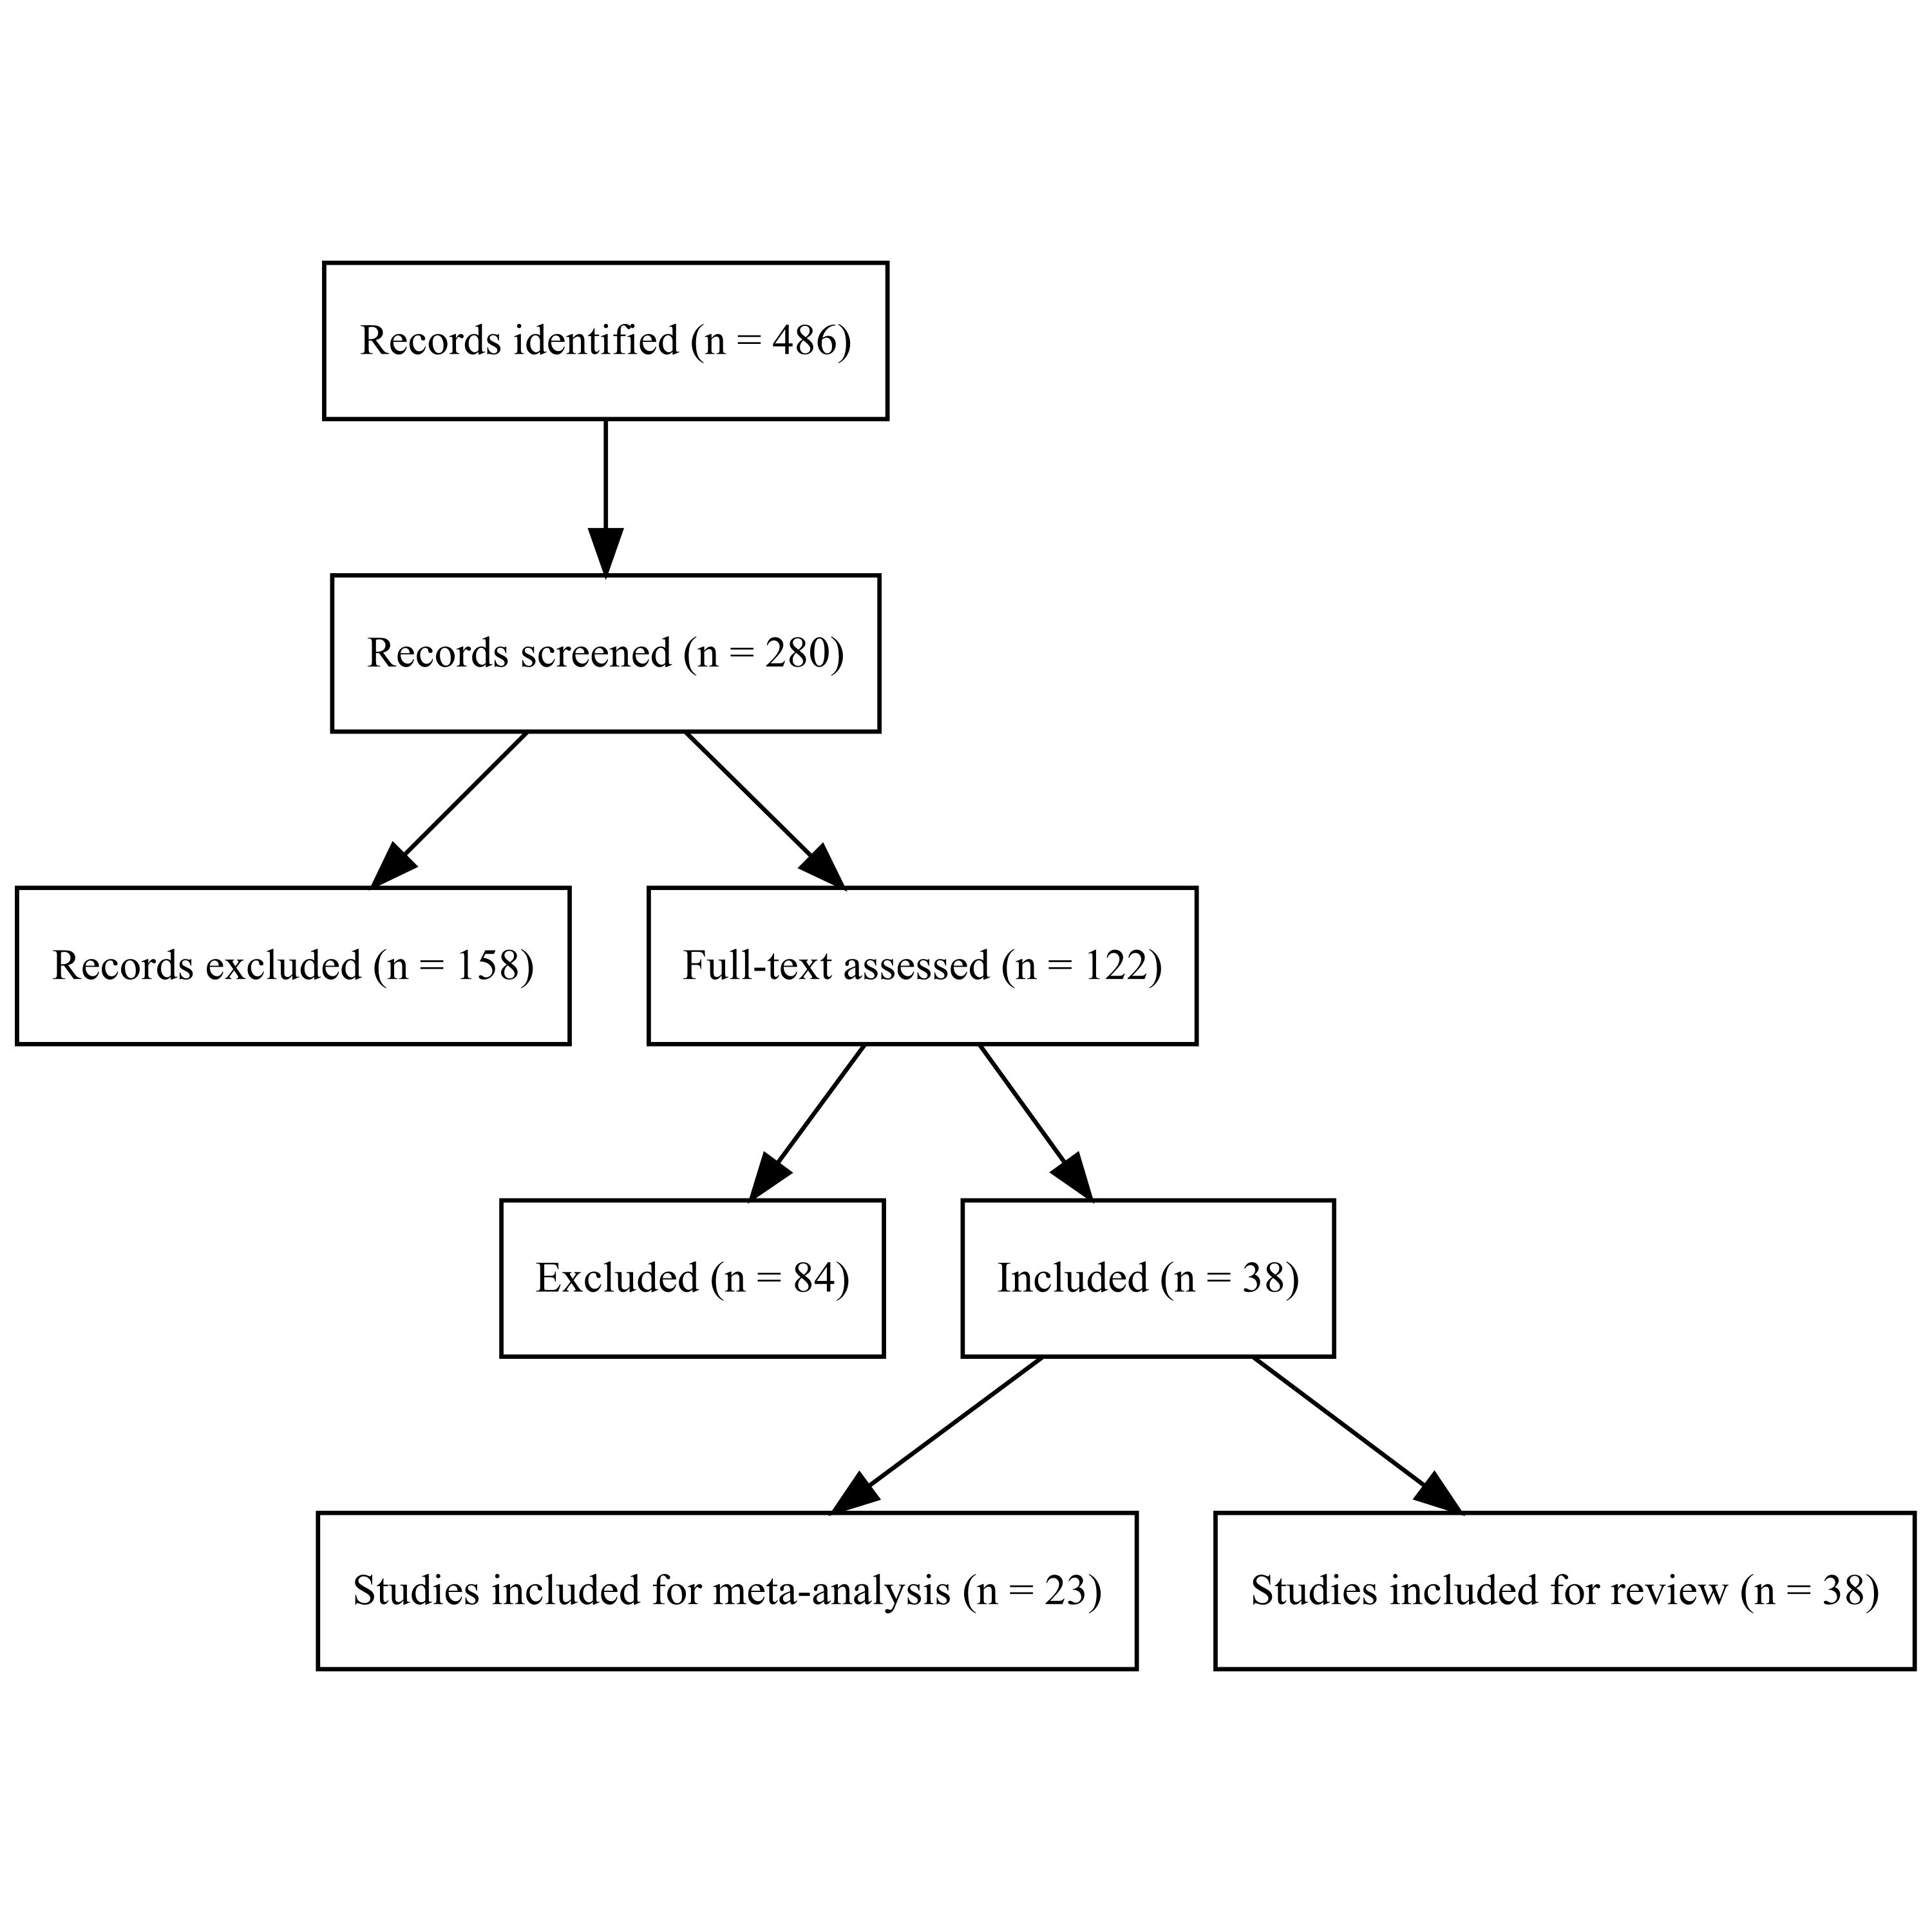
\includegraphics[keepaspectratio]{prisma.png}}

}

\end{figure}%

\begin{table}

{\caption{{Studies included in the review}{\label{tbl-studies-summary}}}
\vspace{-20pt}}

\begin{longtable}[]{@{}
  >{\raggedright\arraybackslash}p{(\linewidth - 12\tabcolsep) * \real{0.1429}}
  >{\raggedright\arraybackslash}p{(\linewidth - 12\tabcolsep) * \real{0.1429}}
  >{\raggedright\arraybackslash}p{(\linewidth - 12\tabcolsep) * \real{0.1429}}
  >{\raggedright\arraybackslash}p{(\linewidth - 12\tabcolsep) * \real{0.1429}}
  >{\raggedright\arraybackslash}p{(\linewidth - 12\tabcolsep) * \real{0.1429}}
  >{\raggedright\arraybackslash}p{(\linewidth - 12\tabcolsep) * \real{0.1429}}
  >{\raggedright\arraybackslash}p{(\linewidth - 12\tabcolsep) * \real{0.1429}}@{}}
\toprule\noalign{}
\begin{minipage}[b]{\linewidth}\raggedright
Authors
\end{minipage} & \begin{minipage}[b]{\linewidth}\raggedright
Year
\end{minipage} & \begin{minipage}[b]{\linewidth}\raggedright
Study design
\end{minipage} & \begin{minipage}[b]{\linewidth}\raggedright
Country
\end{minipage} & \begin{minipage}[b]{\linewidth}\raggedright
n
\end{minipage} & \begin{minipage}[b]{\linewidth}\raggedright
Group
\end{minipage} & \begin{minipage}[b]{\linewidth}\raggedright
Main focus
\end{minipage} \\
\midrule\noalign{}
\endhead
\bottomrule\noalign{}
\endlastfoot
Beatty et al. &
(\citeproc{ref-beattySensePurposeSocialemotionalbehavioral2025}{2025}) &
Cross-sectional & United States & 412 & Young adults & Associations
between sense of purpose and SEB skills in university students \\
Breil et al. & (\citeproc{ref-breil2022}{2022}) & Cross-sectional &
Germany & 137 & Young adults & Associations between self- and observer-
reports for three social skills \\
Chen et al. & (\citeproc{ref-chenSocialEmotionalBehavioral2024}{2024}) &
Cross-sectional & China & 2,992 & Adults & SEB skills and their
incremental validity for job outcomes beyond personality traits \\
Collie \& Ryan & (\citeproc{ref-collie2025}{2025}) & Cross-sectional &
Australia & 373 & Secondary school & Parent-rated SEB skills and their
associations with children perceived socio-emotional competence and
autonomy support \\
De Fruyt et al. &
(\citeproc{ref-defruytChallengesOpportunitiesAssessment2025}{2025}) &
Theoretical & & & & Conceptual and methodological challenges in SEB
skills assessment and interventions \\
Feraco \& Meneghetti &
(\citeproc{ref-feracoSocialEmotionalBehavioral2023}{2023}) &
Cross-sectional & Germany, Italy, Unites States & 4,106 & Secondary
school & Age and gender differences in SEB skills among adolescents \\
Feraco et al. &
(\citeproc{ref-feracoSocialEmotionalBehavioral2025}{2025}) &
Cross-sectional & Italy & 2,965 & Secondary school & SEB skills in
students with learning disabilities \\
Feraco et al. &
(\citeproc{ref-feracoItalianBehavioralEmotional2024}{2024}) &
Cross-sectional & Italy & 1,814 & Secondary school \& Adults &
Validation of the Italian version of the BESSI \\
Feraco et al. & (\citeproc{ref-feracoDifferencesChangeGoals2025}{2025})
& Experimental & Italy, United States & 264 & young\_adult & Change
goals and perceived feasibility about changing SEB skills vs traits \\
Feraco et al. & (\citeproc{ref-feracoRoleSocialEmotional2025}{2025}) &
Cross-sectional & Italy & 702 & Secondary school & Associations between
SEB skills and pro-environmental attitudes and behaviors \\
Feraco et al. & (\citeproc{ref-feracoSoftSkillsHigh2025}{2025}) &
Cross-sectional & Italy & 5,075 & Secondary school & Associations
between SEB skills and self-regulated learning factors \\
Ichsan et al. & (\citeproc{ref-ichsanVirtualRealitySkill2025}{2025}) &
Review & & & & Systematic review on virtual-reality technology for SEB
skills development \\
Lechner \& Urban &
(\citeproc{ref-lechnerInequalitiesAdolescentsSocial2025}{2025}) &
Cross-sectional & Germany & 3,162 & Secondary school & Inequalities in
SEB skills by gender, SES, and migration background \\
Lechner et al. &
(\citeproc{ref-lechnerBehavioralEmotionalSocial2022}{2022}) &
Cross-sectional & Germany & 1,164 & Adults & Validation of the German
version of the BESSI \\
Napolitano et al. &
(\citeproc{ref-napolitanoSocialEmotionalBehavioral2021}{2021}) &
Theoretical & & & & Integrative SEB model and its developmental
importance in adolescence \\
Napolitano et al. &
(\citeproc{ref-napolitanoChangesSocialEmotional2025}{2025}) &
Longitudinal & United States & 942 & Secondary school & Longitudinal
changes in SEB skills and outcomes \\
Pellegrino et al. &
(\citeproc{ref-pellegrinoUniversityStudentsSpecific2026}{2026}) &
Cross-sectional & Italy & 752 & Young adults & Associations between SEB
skills and university students outcomes \\
Pellegrino et al. & (\citeproc{ref-pellegrinoReadyWhatsNext2025}{2025})
& Cross-sectional & Italy & 350 & Secondary school & Associations
between SEB skills and career adaptability \\
Postigo et al. &
(\citeproc{ref-postigoBehavioralEmotionalSocial2024}{2024}) &
Cross-sectional & Spain & 303 & Adults & Validation of the Spanish
version of the BESSI \\
Ringwald et al. & (\citeproc{ref-ringwaldMoreSkillTrait2025}{2025}) &
Cross-sectional & United States & 840 & Secondary school &
Traits--skills (mis)matches and implications for youth outcomes \\
Sewell et al. &
(\citeproc{ref-sewellAssessingSocialEmotional2024a}{2024}) &
Cross-sectional & Germany, United States & 2,792 & Secondary school,
Yound adults, Adults & Development and validation of short BESSI
forms \\
Sewell et al. & (\citeproc{ref-sewell2026}{2026}) & Longitudinal &
United States & 455 & Young adults & Volunteering as predictor of SEB
skills changes \\
Sewell et al. &
(\citeproc{ref-sewellSocialEmotionalBehavioral2023}{2023}) &
Longitudinal & United States & 248 & Young adults & SEB skills as
predictors of volunteering during COVID-19 \\
Sharabi et al. &
(\citeproc{ref-sharabiUndergraduatesAchievementSatisfaction2025}{2025})
& Cross-sectional & Israel, Italy, Spain & 319 & Young adults &
Association between SEB skills and university student outcomes \\
Soto et al. & (\citeproc{ref-sotoWhatWhatCan2023}{2023}) &
Cross-sectional & United States & 975 & Secondary school & SEB skills
and personality traits predicting academic success \\
Soto et al. & (\citeproc{ref-sotoGoingTraitsSocial2024}{2024}) &
Cross-sectional & United States & 897 & Secondary school & Associations
between SEB skills and multiple adolescents'outcomes \\
Soto et al. &
(\citeproc{ref-sotoIntegrativeFrameworkConceptualizing2022}{2022}) &
Cross-sectional & United States & 6,309 & Secondary school, Young
adults, Adults & Validation of the original BESSI \\
Vega-Dienstmaier et al. &
(\citeproc{ref-vega-dienstmaierValidationSelfapplicableVersion2024}{2024})
& Cross-sectional & Peru & 625 & Secondary school & Validation of the
peruvian version of the Resilience Subscale of the BESSI \\
Walton et al. &
(\citeproc{ref-waltonConsiderationsWhenDetermining2024}{2024}) &
Cross-sectional & United States & 474 & Secondary school & Assessment
challenges in differentiating skills vs traits \\
Yoon et al. & (\citeproc{ref-yoonExaminingSEBSkills2024}{2024}) &
Cross-sectional & United States & 642 & Secondary school & SEB skills
and their incremental validity for academic achievement beyond
personality traits \\
\end{longtable}

\end{table}

\subsection{Multilevel Meta-analysis of
Correlations}\label{multilevel-meta-analysis-of-correlations}

As a demonstration of the project's multilevel meta-analytic pipeline,
we tested the associations between the five SEB skill domains and
academic achievement. Following preregistered procedures, a three-level
random-effects model was used, with effects nested within samples and
studies. In line with Borenstein and colleagues
(\citeproc{ref-borenstein2021}{2021}), Fisher's \emph{z} transformations
were applied and then back-transformed to Pearson's \emph{r} for
interpretation. The metafor package was used for the meta-analysis
(\citeproc{ref-viechtbauer2010ConductingMetaanalysesMetafor}{Viechtbauer,
2010}).

\begin{table}

{\caption{{Meta-analytical associations between SEB skills and academic
achievement}{\label{tbl-meta-results}}}
\vspace{-20pt}}

\global\setlength{\Oldarrayrulewidth}{\arrayrulewidth}

\global\setlength{\Oldtabcolsep}{\tabcolsep}

\setlength{\tabcolsep}{2pt}

\renewcommand*{\arraystretch}{1.5}



\providecommand{\ascline}[3]{\noalign{\global\arrayrulewidth #1}\arrayrulecolor[HTML]{#2}\cline{#3}}

\begin{longtable*}[c]{|p{1.55in}|p{0.96in}|p{0.78in}|p{0.90in}|p{0.95in}|p{0.55in}|p{0.73in}|p{0.55in}}



\ascline{0.75pt}{000000}{1-8}

\multicolumn{1}{>{\centering}m{\dimexpr 1.55in+0\tabcolsep}}{\textcolor[HTML]{000000}{\fontsize{11}{22}\selectfont{\global\setmainfont{Times New Roman}{Skill}}}} & \multicolumn{1}{>{\centering}m{\dimexpr 0.96in+0\tabcolsep}}{\textcolor[HTML]{000000}{\fontsize{11}{22}\selectfont{\global\setmainfont{Times New Roman}{N\ (k)}}}} & \multicolumn{1}{>{\centering}m{\dimexpr 0.78in+0\tabcolsep}}{\textcolor[HTML]{000000}{\fontsize{11}{22}\selectfont{\global\setmainfont{Times New Roman}{r}}}} & \multicolumn{1}{>{\centering}m{\dimexpr 0.9in+0\tabcolsep}}{\textcolor[HTML]{000000}{\fontsize{11}{22}\selectfont{\global\setmainfont{Times New Roman}{CI}}}} & \multicolumn{1}{>{\centering}m{\dimexpr 0.95in+0\tabcolsep}}{\textcolor[HTML]{000000}{\fontsize{11}{22}\selectfont{\global\setmainfont{Times New Roman}{PI}}}} & \multicolumn{1}{>{\centering}m{\dimexpr 0.55in+0\tabcolsep}}{\textcolor[HTML]{000000}{\fontsize{11}{22}\selectfont{\global\setmainfont{Times New Roman}{se}}}} & \multicolumn{1}{>{\centering}m{\dimexpr 0.73in+0\tabcolsep}}{\textcolor[HTML]{000000}{\fontsize{11}{22}\selectfont{\global\setmainfont{Times New Roman}{q}}}} & \multicolumn{1}{>{\centering}m{\dimexpr 0.55in+0\tabcolsep}}{\textcolor[HTML]{000000}{\fontsize{11}{22}\selectfont{\global\setmainfont{Times New Roman}{tau2}}}} \\

\ascline{0.75pt}{000000}{1-8}\endfirsthead 

\ascline{0.75pt}{000000}{1-8}

\multicolumn{1}{>{\centering}m{\dimexpr 1.55in+0\tabcolsep}}{\textcolor[HTML]{000000}{\fontsize{11}{22}\selectfont{\global\setmainfont{Times New Roman}{Skill}}}} & \multicolumn{1}{>{\centering}m{\dimexpr 0.96in+0\tabcolsep}}{\textcolor[HTML]{000000}{\fontsize{11}{22}\selectfont{\global\setmainfont{Times New Roman}{N\ (k)}}}} & \multicolumn{1}{>{\centering}m{\dimexpr 0.78in+0\tabcolsep}}{\textcolor[HTML]{000000}{\fontsize{11}{22}\selectfont{\global\setmainfont{Times New Roman}{r}}}} & \multicolumn{1}{>{\centering}m{\dimexpr 0.9in+0\tabcolsep}}{\textcolor[HTML]{000000}{\fontsize{11}{22}\selectfont{\global\setmainfont{Times New Roman}{CI}}}} & \multicolumn{1}{>{\centering}m{\dimexpr 0.95in+0\tabcolsep}}{\textcolor[HTML]{000000}{\fontsize{11}{22}\selectfont{\global\setmainfont{Times New Roman}{PI}}}} & \multicolumn{1}{>{\centering}m{\dimexpr 0.55in+0\tabcolsep}}{\textcolor[HTML]{000000}{\fontsize{11}{22}\selectfont{\global\setmainfont{Times New Roman}{se}}}} & \multicolumn{1}{>{\centering}m{\dimexpr 0.73in+0\tabcolsep}}{\textcolor[HTML]{000000}{\fontsize{11}{22}\selectfont{\global\setmainfont{Times New Roman}{q}}}} & \multicolumn{1}{>{\centering}m{\dimexpr 0.55in+0\tabcolsep}}{\textcolor[HTML]{000000}{\fontsize{11}{22}\selectfont{\global\setmainfont{Times New Roman}{tau2}}}} \\

\ascline{0.75pt}{000000}{1-8}\endhead



\multicolumn{1}{>{\centering}p{\dimexpr 1.55in+0\tabcolsep}}{\textcolor[HTML]{000000}{\fontsize{11}{22}\selectfont{\global\setmainfont{Times New Roman}{Cooperation}}}} & \multicolumn{1}{>{\centering}p{\dimexpr 0.96in+0\tabcolsep}}{\textcolor[HTML]{000000}{\fontsize{11}{22}\selectfont{\global\setmainfont{Times New Roman}{12672\ (10)}}}} & \multicolumn{1}{>{\centering}p{\dimexpr 0.78in+0\tabcolsep}}{\textcolor[HTML]{000000}{\fontsize{11}{22}\selectfont{\global\setmainfont{Times New Roman}{0.10**}}}} & \multicolumn{1}{>{\centering}p{\dimexpr 0.9in+0\tabcolsep}}{\textcolor[HTML]{000000}{\fontsize{11}{22}\selectfont{\global\setmainfont{Times New Roman}{0.03;\ 0.17}}}} & \multicolumn{1}{>{\centering}p{\dimexpr 0.95in+0\tabcolsep}}{\textcolor[HTML]{000000}{\fontsize{11}{22}\selectfont{\global\setmainfont{Times New Roman}{-0.10;\ 0.29}}}} & \multicolumn{1}{>{\centering}p{\dimexpr 0.55in+0\tabcolsep}}{\textcolor[HTML]{000000}{\fontsize{11}{22}\selectfont{\global\setmainfont{Times New Roman}{0.03}}}} & \multicolumn{1}{>{\centering}p{\dimexpr 0.73in+0\tabcolsep}}{\textcolor[HTML]{000000}{\fontsize{11}{22}\selectfont{\global\setmainfont{Times New Roman}{48\ (9)*}}}} & \multicolumn{1}{>{\centering}p{\dimexpr 0.55in+0\tabcolsep}}{\textcolor[HTML]{000000}{\fontsize{11}{22}\selectfont{\global\setmainfont{Times New Roman}{0.01}}}} \\





\multicolumn{1}{>{\centering}p{\dimexpr 1.55in+0\tabcolsep}}{\textcolor[HTML]{000000}{\fontsize{11}{22}\selectfont{\global\setmainfont{Times New Roman}{Emotional\ resilience}}}} & \multicolumn{1}{>{\centering}p{\dimexpr 0.96in+0\tabcolsep}}{\textcolor[HTML]{000000}{\fontsize{11}{22}\selectfont{\global\setmainfont{Times New Roman}{12672\ (10)}}}} & \multicolumn{1}{>{\centering}p{\dimexpr 0.78in+0\tabcolsep}}{\textcolor[HTML]{000000}{\fontsize{11}{22}\selectfont{\global\setmainfont{Times New Roman}{0.06*}}}} & \multicolumn{1}{>{\centering}p{\dimexpr 0.9in+0\tabcolsep}}{\textcolor[HTML]{000000}{\fontsize{11}{22}\selectfont{\global\setmainfont{Times New Roman}{0.01;\ 0.11}}}} & \multicolumn{1}{>{\centering}p{\dimexpr 0.95in+0\tabcolsep}}{\textcolor[HTML]{000000}{\fontsize{11}{22}\selectfont{\global\setmainfont{Times New Roman}{-0.08;\ 0.20}}}} & \multicolumn{1}{>{\centering}p{\dimexpr 0.55in+0\tabcolsep}}{\textcolor[HTML]{000000}{\fontsize{11}{22}\selectfont{\global\setmainfont{Times New Roman}{0.02}}}} & \multicolumn{1}{>{\centering}p{\dimexpr 0.73in+0\tabcolsep}}{\textcolor[HTML]{000000}{\fontsize{11}{22}\selectfont{\global\setmainfont{Times New Roman}{24\ (9)*}}}} & \multicolumn{1}{>{\centering}p{\dimexpr 0.55in+0\tabcolsep}}{\textcolor[HTML]{000000}{\fontsize{11}{22}\selectfont{\global\setmainfont{Times New Roman}{0.00}}}} \\





\multicolumn{1}{>{\centering}p{\dimexpr 1.55in+0\tabcolsep}}{\textcolor[HTML]{000000}{\fontsize{11}{22}\selectfont{\global\setmainfont{Times New Roman}{Innovation}}}} & \multicolumn{1}{>{\centering}p{\dimexpr 0.96in+0\tabcolsep}}{\textcolor[HTML]{000000}{\fontsize{11}{22}\selectfont{\global\setmainfont{Times New Roman}{12672\ (10)}}}} & \multicolumn{1}{>{\centering}p{\dimexpr 0.78in+0\tabcolsep}}{\textcolor[HTML]{000000}{\fontsize{11}{22}\selectfont{\global\setmainfont{Times New Roman}{0.11*}}}} & \multicolumn{1}{>{\centering}p{\dimexpr 0.9in+0\tabcolsep}}{\textcolor[HTML]{000000}{\fontsize{11}{22}\selectfont{\global\setmainfont{Times New Roman}{0.03;\ 0.19}}}} & \multicolumn{1}{>{\centering}p{\dimexpr 0.95in+0\tabcolsep}}{\textcolor[HTML]{000000}{\fontsize{11}{22}\selectfont{\global\setmainfont{Times New Roman}{-0.14;\ 0.35}}}} & \multicolumn{1}{>{\centering}p{\dimexpr 0.55in+0\tabcolsep}}{\textcolor[HTML]{000000}{\fontsize{11}{22}\selectfont{\global\setmainfont{Times New Roman}{0.04}}}} & \multicolumn{1}{>{\centering}p{\dimexpr 0.73in+0\tabcolsep}}{\textcolor[HTML]{000000}{\fontsize{11}{22}\selectfont{\global\setmainfont{Times New Roman}{86\ (9)*}}}} & \multicolumn{1}{>{\centering}p{\dimexpr 0.55in+0\tabcolsep}}{\textcolor[HTML]{000000}{\fontsize{11}{22}\selectfont{\global\setmainfont{Times New Roman}{0.01}}}} \\





\multicolumn{1}{>{\centering}p{\dimexpr 1.55in+0\tabcolsep}}{\textcolor[HTML]{000000}{\fontsize{11}{22}\selectfont{\global\setmainfont{Times New Roman}{Self-management}}}} & \multicolumn{1}{>{\centering}p{\dimexpr 0.96in+0\tabcolsep}}{\textcolor[HTML]{000000}{\fontsize{11}{22}\selectfont{\global\setmainfont{Times New Roman}{12672\ (10)}}}} & \multicolumn{1}{>{\centering}p{\dimexpr 0.78in+0\tabcolsep}}{\textcolor[HTML]{000000}{\fontsize{11}{22}\selectfont{\global\setmainfont{Times New Roman}{0.24***}}}} & \multicolumn{1}{>{\centering}p{\dimexpr 0.9in+0\tabcolsep}}{\textcolor[HTML]{000000}{\fontsize{11}{22}\selectfont{\global\setmainfont{Times New Roman}{0.18;\ 0.30}}}} & \multicolumn{1}{>{\centering}p{\dimexpr 0.95in+0\tabcolsep}}{\textcolor[HTML]{000000}{\fontsize{11}{22}\selectfont{\global\setmainfont{Times New Roman}{\ 0.04;\ 0.42}}}} & \multicolumn{1}{>{\centering}p{\dimexpr 0.55in+0\tabcolsep}}{\textcolor[HTML]{000000}{\fontsize{11}{22}\selectfont{\global\setmainfont{Times New Roman}{0.03}}}} & \multicolumn{1}{>{\centering}p{\dimexpr 0.73in+0\tabcolsep}}{\textcolor[HTML]{000000}{\fontsize{11}{22}\selectfont{\global\setmainfont{Times New Roman}{59\ (9)*}}}} & \multicolumn{1}{>{\centering}p{\dimexpr 0.55in+0\tabcolsep}}{\textcolor[HTML]{000000}{\fontsize{11}{22}\selectfont{\global\setmainfont{Times New Roman}{0.01}}}} \\





\multicolumn{1}{>{\centering}p{\dimexpr 1.55in+0\tabcolsep}}{\textcolor[HTML]{000000}{\fontsize{11}{22}\selectfont{\global\setmainfont{Times New Roman}{Social\ engagement}}}} & \multicolumn{1}{>{\centering}p{\dimexpr 0.96in+0\tabcolsep}}{\textcolor[HTML]{000000}{\fontsize{11}{22}\selectfont{\global\setmainfont{Times New Roman}{12672\ (10)}}}} & \multicolumn{1}{>{\centering}p{\dimexpr 0.78in+0\tabcolsep}}{\textcolor[HTML]{000000}{\fontsize{11}{22}\selectfont{\global\setmainfont{Times New Roman}{0.11**}}}} & \multicolumn{1}{>{\centering}p{\dimexpr 0.9in+0\tabcolsep}}{\textcolor[HTML]{000000}{\fontsize{11}{22}\selectfont{\global\setmainfont{Times New Roman}{0.04;\ 0.17}}}} & \multicolumn{1}{>{\centering}p{\dimexpr 0.95in+0\tabcolsep}}{\textcolor[HTML]{000000}{\fontsize{11}{22}\selectfont{\global\setmainfont{Times New Roman}{-0.08;\ 0.29}}}} & \multicolumn{1}{>{\centering}p{\dimexpr 0.55in+0\tabcolsep}}{\textcolor[HTML]{000000}{\fontsize{11}{22}\selectfont{\global\setmainfont{Times New Roman}{0.03}}}} & \multicolumn{1}{>{\centering}p{\dimexpr 0.73in+0\tabcolsep}}{\textcolor[HTML]{000000}{\fontsize{11}{22}\selectfont{\global\setmainfont{Times New Roman}{38\ (9)*}}}} & \multicolumn{1}{>{\centering}p{\dimexpr 0.55in+0\tabcolsep}}{\textcolor[HTML]{000000}{\fontsize{11}{22}\selectfont{\global\setmainfont{Times New Roman}{0.01}}}} \\

\ascline{0.75pt}{000000}{1-8}



\end{longtable*}



\arrayrulecolor[HTML]{000000}

\global\setlength{\arrayrulewidth}{\Oldarrayrulewidth}

\global\setlength{\tabcolsep}{\Oldtabcolsep}

\renewcommand*{\arraystretch}{1}

{\vspace{-20pt}
\noindent \emph{Note.} * \emph{p} \textless{} .05; ** \emph{p}
\textless{} .01; *** \emph{p} \textless{} .001; CI = Confidence
intervals; PI = Prediction intervals; se = Standard error}

\end{table}

\begin{figure}

\caption{\label{fig-meta-analysis-plot}Meta-analytical associations
between the five SEB domains and academic achievement.}

\centering{

\pandocbounded{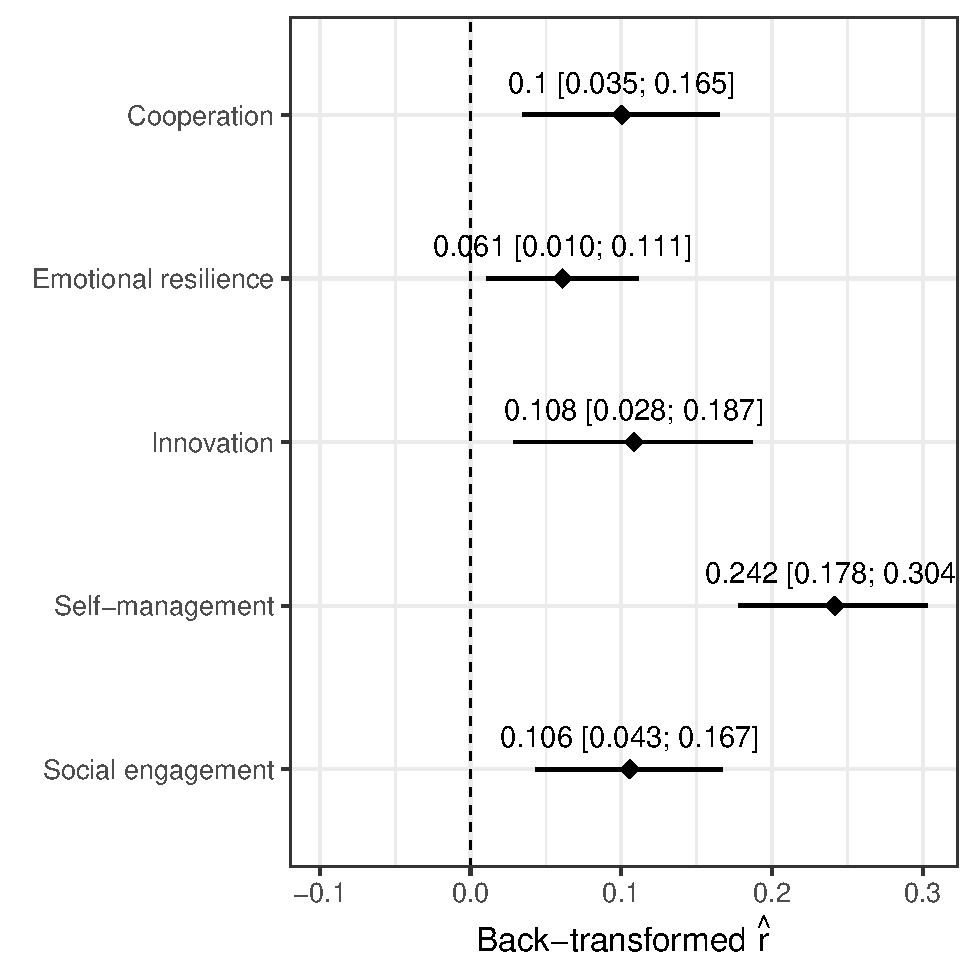
\includegraphics[keepaspectratio]{livingSEBpaper_files/figure-pdf/fig-meta-analysis-plot-1.pdf}}

}

\end{figure}%

A total of 50 effect sizes from 9 studies and 10 samples were included.
For each SEB domain, the median available sample size was 796 (minimum
sample size = 319; maximum sample size = 5075).

The full set of results is available in Table~\ref{tbl-meta-results} and
Figure~\ref{fig-meta-analysis-plot}. Of the five meta-analysed
correlations with academic achievement, four were larger than 0.10, with
significant effects (p \textless{} 0.01) ranging between 0.1 (i.e.,
Cooperation) and 0.24 (i.e., Self-management).

The \emph{Q} test for heterogeneity shows that there is significant
heterogeneity across studies, with the standard deviation of the effects
ranging between 0.06 and 0.11.

These results suggest that, with the exception of Emotional resilience
skills, each SEB skill might be considered as a positive correlate of
academic achievement, though most effects are small in magnitude.
Indeed, only Self-management skills show correlations larger than 0.20
with academic achievement.

\subsection{Meta-analytic Structural Equation
Modeling}\label{meta-analytic-structural-equation-modeling}

To illustrate the use of meta-analytic structural equation modeling
within the \emph{Living SEB Skills Project}, we tested whether each SEB
skill predicted academic achievement beyond their corresponding Big Five
traits and other SEB skills. First, using the first stage of the
two-staged structural equation modelling (TSSEM) procedure, we
synthesized the bivariate correlations among all variables using a
random-effects model. This yields a pooled meta-analytic correlation
matrix of each pairwise association between all the Big Five traits, the
five SEB domains, and academic achievement that accounts for sampling
error and between-study heterogeneity
(\citeproc{ref-cheung2015MetaAnalysisStructuralEquation}{Cheung, 2015}).

Next, we applied one-stage meta-analytic structural equation modelling
(OSMASEM) (\citeproc{ref-jak2020MetaanalyticStructuralEquation}{Jak \&
Cheung, 2020}). OSMASEM estimates the structural model in a single step
by fitting a structural equation model directly to the meta-analytic
covariance structure while simultaneously modeling sampling variance and
between-study heterogeneity. This approach allows regression paths to be
estimated within an SEM framework using the full pooled covariance
matrix. Using OSMASEM, we estimated five saturated regression models,
each including one SEB domain and its matched Big Five trait as
predictors of academic achievement. Additionally, a multiple regression
model was estimated including all five SEB domains as predictors of
academic achievement.

The metaSEM (\citeproc{ref-cheung2024MetaSEMMetaAnalysisUsing}{Cheung,
2024}) and lavaan
(\citeproc{ref-rosseel2012LavaanPackageStructural}{Rosseel, 2012}) R
packages were used for these analysis and the open code of the webMASEM
app (\citeproc{ref-jak2021MetaanalyticStructuralEquation}{Jak et al.,
2021}) was used to guide coding of the \emph{Living SEB App} section for
MASEM.

MASEM analyses were based on varying number of effect sizes per pairwise
correlation (i.e., different correlation matrices), with the minimum
available effects per correlation being 3 and the maximum being 25. As a
consequence, also sample sizes and precision differed, with the minimum
being 2712 (i.e., correlations between personality traits and academic
achievement) and the maximum being 23321 (i.e., correlations between SEB
domains). Correlation matrices were taken from 26 samples included in 19
different studies.

Given the low number of studies available for some variables, we set
between-study variance to zero and estimated a common effect across
studies. This approach avoids attempting to estimate random‐effects
components that would be unstable or poorly identified in sparse
conditions.

\subsubsection{Pooled correlations}\label{pooled-correlations}

\begin{figure}

\caption{\label{fig-corrplot}Pooled correlation matrix}

\centering{

\pandocbounded{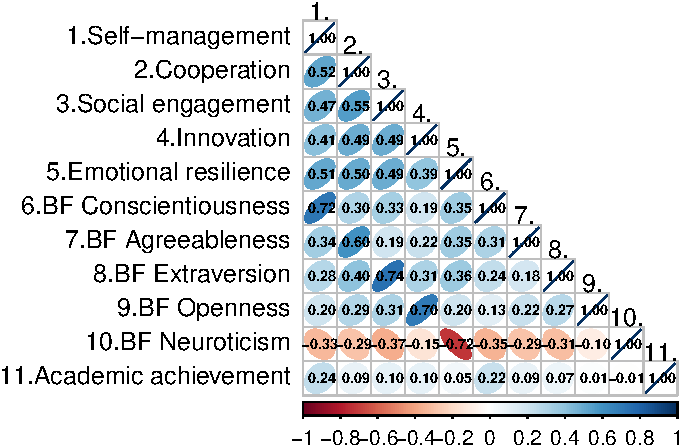
\includegraphics[keepaspectratio]{livingSEBpaper_files/figure-pdf/fig-corrplot-1.pdf}}

}

\end{figure}%

The pooled correlation matrix is reported in Figure~\ref{fig-corrplot}.
As clear from the diagonal cells linking each skill to the corresponding
trait, their correlation is substantial (\emph{r} \textgreater{} 0.6),
with the highest correlation reaching 0.74. For what concerns academic
achievement, Self-management (r = 0.24), BF Conscientiousness (r = 0.22)
were the only variables among SEB skills and Big Five traits showing a
pooled correlation higher than \emph{r} \textgreater{} 0.2 with academic
achievement.

\subsubsection{Incremental Validity Beyond the Big
Five}\label{incremental-validity-beyond-the-big-five}

\begin{table}

{\caption{{OSMASEM regression and correlation coefficients for the five
models}{\label{tbl-osmasem-summary}}}
\vspace{-20pt}}

\global\setlength{\Oldarrayrulewidth}{\arrayrulewidth}

\global\setlength{\Oldtabcolsep}{\tabcolsep}

\setlength{\tabcolsep}{2pt}

\renewcommand*{\arraystretch}{1.5}



\providecommand{\ascline}[3]{\noalign{\global\arrayrulewidth #1}\arrayrulecolor[HTML]{#2}\cline{#3}}

\begin{longtable*}[c]{|p{1.44in}|p{0.29in}|p{1.37in}|p{0.70in}|p{0.38in}|p{0.88in}|p{0.57in}}



\ascline{0.75pt}{000000}{1-7}

\multicolumn{1}{>{\centering}m{\dimexpr 1.44in+0\tabcolsep}}{\textcolor[HTML]{000000}{\fontsize{10}{20}\selectfont{\global\setmainfont{Times New Roman}{Outcome}}}} & \multicolumn{1}{>{\centering}m{\dimexpr 0.29in+0\tabcolsep}}{\textcolor[HTML]{000000}{\fontsize{10}{20}\selectfont{\global\setmainfont{Times New Roman}{}}}} & \multicolumn{1}{>{\centering}m{\dimexpr 1.37in+0\tabcolsep}}{\textcolor[HTML]{000000}{\fontsize{10}{20}\selectfont{\global\setmainfont{Times New Roman}{Predictor}}}} & \multicolumn{1}{>{\centering}m{\dimexpr 0.7in+0\tabcolsep}}{\textcolor[HTML]{000000}{\fontsize{10}{20}\selectfont{\global\setmainfont{Times New Roman}{Estimate}}}} & \multicolumn{1}{>{\centering}m{\dimexpr 0.38in+0\tabcolsep}}{\textcolor[HTML]{000000}{\fontsize{10}{20}\selectfont{\global\setmainfont{Times New Roman}{se}}}} & \multicolumn{1}{>{\centering}m{\dimexpr 0.88in+0\tabcolsep}}{\textcolor[HTML]{000000}{\fontsize{10}{20}\selectfont{\global\setmainfont{Times New Roman}{CI}}}} & \multicolumn{1}{>{\centering}m{\dimexpr 0.57in+0\tabcolsep}}{\textcolor[HTML]{000000}{\fontsize{10}{20}\selectfont{\global\setmainfont{Times New Roman}{z}}}} \\

\ascline{0.75pt}{000000}{1-7}\endfirsthead 

\ascline{0.75pt}{000000}{1-7}

\multicolumn{1}{>{\centering}m{\dimexpr 1.44in+0\tabcolsep}}{\textcolor[HTML]{000000}{\fontsize{10}{20}\selectfont{\global\setmainfont{Times New Roman}{Outcome}}}} & \multicolumn{1}{>{\centering}m{\dimexpr 0.29in+0\tabcolsep}}{\textcolor[HTML]{000000}{\fontsize{10}{20}\selectfont{\global\setmainfont{Times New Roman}{}}}} & \multicolumn{1}{>{\centering}m{\dimexpr 1.37in+0\tabcolsep}}{\textcolor[HTML]{000000}{\fontsize{10}{20}\selectfont{\global\setmainfont{Times New Roman}{Predictor}}}} & \multicolumn{1}{>{\centering}m{\dimexpr 0.7in+0\tabcolsep}}{\textcolor[HTML]{000000}{\fontsize{10}{20}\selectfont{\global\setmainfont{Times New Roman}{Estimate}}}} & \multicolumn{1}{>{\centering}m{\dimexpr 0.38in+0\tabcolsep}}{\textcolor[HTML]{000000}{\fontsize{10}{20}\selectfont{\global\setmainfont{Times New Roman}{se}}}} & \multicolumn{1}{>{\centering}m{\dimexpr 0.88in+0\tabcolsep}}{\textcolor[HTML]{000000}{\fontsize{10}{20}\selectfont{\global\setmainfont{Times New Roman}{CI}}}} & \multicolumn{1}{>{\centering}m{\dimexpr 0.57in+0\tabcolsep}}{\textcolor[HTML]{000000}{\fontsize{10}{20}\selectfont{\global\setmainfont{Times New Roman}{z}}}} \\

\ascline{0.75pt}{000000}{1-7}\endhead



\multicolumn{1}{>{\centering}p{\dimexpr 1.44in+0\tabcolsep}}{\textcolor[HTML]{000000}{\fontsize{10}{20}\selectfont{\global\setmainfont{Times New Roman}{Academic\ achievement}}}} & \multicolumn{1}{>{\centering}p{\dimexpr 0.29in+0\tabcolsep}}{\textcolor[HTML]{000000}{\fontsize{10}{20}\selectfont{\global\setmainfont{Times New Roman}{\textasciitilde }}}} & \multicolumn{1}{>{\centering}p{\dimexpr 1.37in+0\tabcolsep}}{\textcolor[HTML]{000000}{\fontsize{10}{20}\selectfont{\global\setmainfont{Times New Roman}{BF\ Openness}}}} & \multicolumn{1}{>{\centering}p{\dimexpr 0.7in+0\tabcolsep}}{\textcolor[HTML]{000000}{\fontsize{10}{20}\selectfont{\global\setmainfont{Times New Roman}{-0.065*}}}} & \multicolumn{1}{>{\centering}p{\dimexpr 0.38in+0\tabcolsep}}{\textcolor[HTML]{000000}{\fontsize{10}{20}\selectfont{\global\setmainfont{Times New Roman}{0.03}}}} & \multicolumn{1}{>{\centering}p{\dimexpr 0.88in+0\tabcolsep}}{\textcolor[HTML]{000000}{\fontsize{10}{20}\selectfont{\global\setmainfont{Times New Roman}{[-0.11;\ -0.01]}}}} & \multicolumn{1}{>{\centering}p{\dimexpr 0.57in+0\tabcolsep}}{\textcolor[HTML]{000000}{\fontsize{10}{20}\selectfont{\global\setmainfont{Times New Roman}{-2.55}}}} \\





\multicolumn{1}{>{\centering}p{\dimexpr 1.44in+0\tabcolsep}}{\textcolor[HTML]{000000}{\fontsize{10}{20}\selectfont{\global\setmainfont{Times New Roman}{Academic\ achievement}}}} & \multicolumn{1}{>{\centering}p{\dimexpr 0.29in+0\tabcolsep}}{\textcolor[HTML]{000000}{\fontsize{10}{20}\selectfont{\global\setmainfont{Times New Roman}{\textasciitilde }}}} & \multicolumn{1}{>{\centering}p{\dimexpr 1.37in+0\tabcolsep}}{\textcolor[HTML]{000000}{\fontsize{10}{20}\selectfont{\global\setmainfont{Times New Roman}{Innovation}}}} & \multicolumn{1}{>{\centering}p{\dimexpr 0.7in+0\tabcolsep}}{\textcolor[HTML]{000000}{\fontsize{10}{20}\selectfont{\global\setmainfont{Times New Roman}{0.16***}}}} & \multicolumn{1}{>{\centering}p{\dimexpr 0.38in+0\tabcolsep}}{\textcolor[HTML]{000000}{\fontsize{10}{20}\selectfont{\global\setmainfont{Times New Roman}{0.02}}}} & \multicolumn{1}{>{\centering}p{\dimexpr 0.88in+0\tabcolsep}}{\textcolor[HTML]{000000}{\fontsize{10}{20}\selectfont{\global\setmainfont{Times New Roman}{[0.12;\ 0.2]}}}} & \multicolumn{1}{>{\centering}p{\dimexpr 0.57in+0\tabcolsep}}{\textcolor[HTML]{000000}{\fontsize{10}{20}\selectfont{\global\setmainfont{Times New Roman}{8.40}}}} \\





\multicolumn{1}{>{\centering}p{\dimexpr 1.44in+0\tabcolsep}}{\textcolor[HTML]{000000}{\fontsize{10}{20}\selectfont{\global\setmainfont{Times New Roman}{BF\ Openness}}}} & \multicolumn{1}{>{\centering}p{\dimexpr 0.29in+0\tabcolsep}}{\textcolor[HTML]{000000}{\fontsize{10}{20}\selectfont{\global\setmainfont{Times New Roman}{\textasciitilde \textasciitilde }}}} & \multicolumn{1}{>{\centering}p{\dimexpr 1.37in+0\tabcolsep}}{\textcolor[HTML]{000000}{\fontsize{10}{20}\selectfont{\global\setmainfont{Times New Roman}{Innovation}}}} & \multicolumn{1}{>{\centering}p{\dimexpr 0.7in+0\tabcolsep}}{\textcolor[HTML]{000000}{\fontsize{10}{20}\selectfont{\global\setmainfont{Times New Roman}{0.673***}}}} & \multicolumn{1}{>{\centering}p{\dimexpr 0.38in+0\tabcolsep}}{\textcolor[HTML]{000000}{\fontsize{10}{20}\selectfont{\global\setmainfont{Times New Roman}{0.01}}}} & \multicolumn{1}{>{\centering}p{\dimexpr 0.88in+0\tabcolsep}}{\textcolor[HTML]{000000}{\fontsize{10}{20}\selectfont{\global\setmainfont{Times New Roman}{[0.66;\ 0.69]}}}} & \multicolumn{1}{>{\centering}p{\dimexpr 0.57in+0\tabcolsep}}{\textcolor[HTML]{000000}{\fontsize{10}{20}\selectfont{\global\setmainfont{Times New Roman}{113.17}}}} \\





\multicolumn{1}{>{\centering}p{\dimexpr 1.44in+0\tabcolsep}}{\textcolor[HTML]{000000}{\fontsize{10}{20}\selectfont{\global\setmainfont{Times New Roman}{Academic\ achievement}}}} & \multicolumn{1}{>{\centering}p{\dimexpr 0.29in+0\tabcolsep}}{\textcolor[HTML]{000000}{\fontsize{10}{20}\selectfont{\global\setmainfont{Times New Roman}{\textasciitilde }}}} & \multicolumn{1}{>{\centering}p{\dimexpr 1.37in+0\tabcolsep}}{\textcolor[HTML]{000000}{\fontsize{10}{20}\selectfont{\global\setmainfont{Times New Roman}{BF\ Conscientiousness}}}} & \multicolumn{1}{>{\centering}p{\dimexpr 0.7in+0\tabcolsep}}{\textcolor[HTML]{000000}{\fontsize{10}{20}\selectfont{\global\setmainfont{Times New Roman}{0.129***}}}} & \multicolumn{1}{>{\centering}p{\dimexpr 0.38in+0\tabcolsep}}{\textcolor[HTML]{000000}{\fontsize{10}{20}\selectfont{\global\setmainfont{Times New Roman}{0.03}}}} & \multicolumn{1}{>{\centering}p{\dimexpr 0.88in+0\tabcolsep}}{\textcolor[HTML]{000000}{\fontsize{10}{20}\selectfont{\global\setmainfont{Times New Roman}{[0.08;\ 0.18]}}}} & \multicolumn{1}{>{\centering}p{\dimexpr 0.57in+0\tabcolsep}}{\textcolor[HTML]{000000}{\fontsize{10}{20}\selectfont{\global\setmainfont{Times New Roman}{4.96}}}} \\





\multicolumn{1}{>{\centering}p{\dimexpr 1.44in+0\tabcolsep}}{\textcolor[HTML]{000000}{\fontsize{10}{20}\selectfont{\global\setmainfont{Times New Roman}{Academic\ achievement}}}} & \multicolumn{1}{>{\centering}p{\dimexpr 0.29in+0\tabcolsep}}{\textcolor[HTML]{000000}{\fontsize{10}{20}\selectfont{\global\setmainfont{Times New Roman}{\textasciitilde }}}} & \multicolumn{1}{>{\centering}p{\dimexpr 1.37in+0\tabcolsep}}{\textcolor[HTML]{000000}{\fontsize{10}{20}\selectfont{\global\setmainfont{Times New Roman}{Self-management}}}} & \multicolumn{1}{>{\centering}p{\dimexpr 0.7in+0\tabcolsep}}{\textcolor[HTML]{000000}{\fontsize{10}{20}\selectfont{\global\setmainfont{Times New Roman}{0.17***}}}} & \multicolumn{1}{>{\centering}p{\dimexpr 0.38in+0\tabcolsep}}{\textcolor[HTML]{000000}{\fontsize{10}{20}\selectfont{\global\setmainfont{Times New Roman}{0.02}}}} & \multicolumn{1}{>{\centering}p{\dimexpr 0.88in+0\tabcolsep}}{\textcolor[HTML]{000000}{\fontsize{10}{20}\selectfont{\global\setmainfont{Times New Roman}{[0.13;\ 0.21]}}}} & \multicolumn{1}{>{\centering}p{\dimexpr 0.57in+0\tabcolsep}}{\textcolor[HTML]{000000}{\fontsize{10}{20}\selectfont{\global\setmainfont{Times New Roman}{8.53}}}} \\





\multicolumn{1}{>{\centering}p{\dimexpr 1.44in+0\tabcolsep}}{\textcolor[HTML]{000000}{\fontsize{10}{20}\selectfont{\global\setmainfont{Times New Roman}{Self-management}}}} & \multicolumn{1}{>{\centering}p{\dimexpr 0.29in+0\tabcolsep}}{\textcolor[HTML]{000000}{\fontsize{10}{20}\selectfont{\global\setmainfont{Times New Roman}{\textasciitilde \textasciitilde }}}} & \multicolumn{1}{>{\centering}p{\dimexpr 1.37in+0\tabcolsep}}{\textcolor[HTML]{000000}{\fontsize{10}{20}\selectfont{\global\setmainfont{Times New Roman}{BF\ Conscientiousness}}}} & \multicolumn{1}{>{\centering}p{\dimexpr 0.7in+0\tabcolsep}}{\textcolor[HTML]{000000}{\fontsize{10}{20}\selectfont{\global\setmainfont{Times New Roman}{0.696***}}}} & \multicolumn{1}{>{\centering}p{\dimexpr 0.38in+0\tabcolsep}}{\textcolor[HTML]{000000}{\fontsize{10}{20}\selectfont{\global\setmainfont{Times New Roman}{0.01}}}} & \multicolumn{1}{>{\centering}p{\dimexpr 0.88in+0\tabcolsep}}{\textcolor[HTML]{000000}{\fontsize{10}{20}\selectfont{\global\setmainfont{Times New Roman}{[0.69;\ 0.71]}}}} & \multicolumn{1}{>{\centering}p{\dimexpr 0.57in+0\tabcolsep}}{\textcolor[HTML]{000000}{\fontsize{10}{20}\selectfont{\global\setmainfont{Times New Roman}{123.48}}}} \\





\multicolumn{1}{>{\centering}p{\dimexpr 1.44in+0\tabcolsep}}{\textcolor[HTML]{000000}{\fontsize{10}{20}\selectfont{\global\setmainfont{Times New Roman}{Academic\ achievement}}}} & \multicolumn{1}{>{\centering}p{\dimexpr 0.29in+0\tabcolsep}}{\textcolor[HTML]{000000}{\fontsize{10}{20}\selectfont{\global\setmainfont{Times New Roman}{\textasciitilde }}}} & \multicolumn{1}{>{\centering}p{\dimexpr 1.37in+0\tabcolsep}}{\textcolor[HTML]{000000}{\fontsize{10}{20}\selectfont{\global\setmainfont{Times New Roman}{BF\ Extraversion}}}} & \multicolumn{1}{>{\centering}p{\dimexpr 0.7in+0\tabcolsep}}{\textcolor[HTML]{000000}{\fontsize{10}{20}\selectfont{\global\setmainfont{Times New Roman}{-0.02}}}} & \multicolumn{1}{>{\centering}p{\dimexpr 0.38in+0\tabcolsep}}{\textcolor[HTML]{000000}{\fontsize{10}{20}\selectfont{\global\setmainfont{Times New Roman}{0.03}}}} & \multicolumn{1}{>{\centering}p{\dimexpr 0.88in+0\tabcolsep}}{\textcolor[HTML]{000000}{\fontsize{10}{20}\selectfont{\global\setmainfont{Times New Roman}{[-0.07;\ 0.03]}}}} & \multicolumn{1}{>{\centering}p{\dimexpr 0.57in+0\tabcolsep}}{\textcolor[HTML]{000000}{\fontsize{10}{20}\selectfont{\global\setmainfont{Times New Roman}{-0.71}}}} \\





\multicolumn{1}{>{\centering}p{\dimexpr 1.44in+0\tabcolsep}}{\textcolor[HTML]{000000}{\fontsize{10}{20}\selectfont{\global\setmainfont{Times New Roman}{Academic\ achievement}}}} & \multicolumn{1}{>{\centering}p{\dimexpr 0.29in+0\tabcolsep}}{\textcolor[HTML]{000000}{\fontsize{10}{20}\selectfont{\global\setmainfont{Times New Roman}{\textasciitilde }}}} & \multicolumn{1}{>{\centering}p{\dimexpr 1.37in+0\tabcolsep}}{\textcolor[HTML]{000000}{\fontsize{10}{20}\selectfont{\global\setmainfont{Times New Roman}{Social\ engagement}}}} & \multicolumn{1}{>{\centering}p{\dimexpr 0.7in+0\tabcolsep}}{\textcolor[HTML]{000000}{\fontsize{10}{20}\selectfont{\global\setmainfont{Times New Roman}{0.115***}}}} & \multicolumn{1}{>{\centering}p{\dimexpr 0.38in+0\tabcolsep}}{\textcolor[HTML]{000000}{\fontsize{10}{20}\selectfont{\global\setmainfont{Times New Roman}{0.02}}}} & \multicolumn{1}{>{\centering}p{\dimexpr 0.88in+0\tabcolsep}}{\textcolor[HTML]{000000}{\fontsize{10}{20}\selectfont{\global\setmainfont{Times New Roman}{[0.07;\ 0.16]}}}} & \multicolumn{1}{>{\centering}p{\dimexpr 0.57in+0\tabcolsep}}{\textcolor[HTML]{000000}{\fontsize{10}{20}\selectfont{\global\setmainfont{Times New Roman}{5.34}}}} \\





\multicolumn{1}{>{\centering}p{\dimexpr 1.44in+0\tabcolsep}}{\textcolor[HTML]{000000}{\fontsize{10}{20}\selectfont{\global\setmainfont{Times New Roman}{Social\ engagement}}}} & \multicolumn{1}{>{\centering}p{\dimexpr 0.29in+0\tabcolsep}}{\textcolor[HTML]{000000}{\fontsize{10}{20}\selectfont{\global\setmainfont{Times New Roman}{\textasciitilde \textasciitilde }}}} & \multicolumn{1}{>{\centering}p{\dimexpr 1.37in+0\tabcolsep}}{\textcolor[HTML]{000000}{\fontsize{10}{20}\selectfont{\global\setmainfont{Times New Roman}{BF\ Extraversion}}}} & \multicolumn{1}{>{\centering}p{\dimexpr 0.7in+0\tabcolsep}}{\textcolor[HTML]{000000}{\fontsize{10}{20}\selectfont{\global\setmainfont{Times New Roman}{0.72***}}}} & \multicolumn{1}{>{\centering}p{\dimexpr 0.38in+0\tabcolsep}}{\textcolor[HTML]{000000}{\fontsize{10}{20}\selectfont{\global\setmainfont{Times New Roman}{0.01}}}} & \multicolumn{1}{>{\centering}p{\dimexpr 0.88in+0\tabcolsep}}{\textcolor[HTML]{000000}{\fontsize{10}{20}\selectfont{\global\setmainfont{Times New Roman}{[0.71;\ 0.73]}}}} & \multicolumn{1}{>{\centering}p{\dimexpr 0.57in+0\tabcolsep}}{\textcolor[HTML]{000000}{\fontsize{10}{20}\selectfont{\global\setmainfont{Times New Roman}{137.88}}}} \\





\multicolumn{1}{>{\centering}p{\dimexpr 1.44in+0\tabcolsep}}{\textcolor[HTML]{000000}{\fontsize{10}{20}\selectfont{\global\setmainfont{Times New Roman}{Academic\ achievement}}}} & \multicolumn{1}{>{\centering}p{\dimexpr 0.29in+0\tabcolsep}}{\textcolor[HTML]{000000}{\fontsize{10}{20}\selectfont{\global\setmainfont{Times New Roman}{\textasciitilde }}}} & \multicolumn{1}{>{\centering}p{\dimexpr 1.37in+0\tabcolsep}}{\textcolor[HTML]{000000}{\fontsize{10}{20}\selectfont{\global\setmainfont{Times New Roman}{BF\ Agreeableness}}}} & \multicolumn{1}{>{\centering}p{\dimexpr 0.7in+0\tabcolsep}}{\textcolor[HTML]{000000}{\fontsize{10}{20}\selectfont{\global\setmainfont{Times New Roman}{0.066**}}}} & \multicolumn{1}{>{\centering}p{\dimexpr 0.38in+0\tabcolsep}}{\textcolor[HTML]{000000}{\fontsize{10}{20}\selectfont{\global\setmainfont{Times New Roman}{0.02}}}} & \multicolumn{1}{>{\centering}p{\dimexpr 0.88in+0\tabcolsep}}{\textcolor[HTML]{000000}{\fontsize{10}{20}\selectfont{\global\setmainfont{Times New Roman}{[0.02;\ 0.11]}}}} & \multicolumn{1}{>{\centering}p{\dimexpr 0.57in+0\tabcolsep}}{\textcolor[HTML]{000000}{\fontsize{10}{20}\selectfont{\global\setmainfont{Times New Roman}{2.80}}}} \\





\multicolumn{1}{>{\centering}p{\dimexpr 1.44in+0\tabcolsep}}{\textcolor[HTML]{000000}{\fontsize{10}{20}\selectfont{\global\setmainfont{Times New Roman}{Academic\ achievement}}}} & \multicolumn{1}{>{\centering}p{\dimexpr 0.29in+0\tabcolsep}}{\textcolor[HTML]{000000}{\fontsize{10}{20}\selectfont{\global\setmainfont{Times New Roman}{\textasciitilde }}}} & \multicolumn{1}{>{\centering}p{\dimexpr 1.37in+0\tabcolsep}}{\textcolor[HTML]{000000}{\fontsize{10}{20}\selectfont{\global\setmainfont{Times New Roman}{Cooperation}}}} & \multicolumn{1}{>{\centering}p{\dimexpr 0.7in+0\tabcolsep}}{\textcolor[HTML]{000000}{\fontsize{10}{20}\selectfont{\global\setmainfont{Times New Roman}{0.052**}}}} & \multicolumn{1}{>{\centering}p{\dimexpr 0.38in+0\tabcolsep}}{\textcolor[HTML]{000000}{\fontsize{10}{20}\selectfont{\global\setmainfont{Times New Roman}{0.02}}}} & \multicolumn{1}{>{\centering}p{\dimexpr 0.88in+0\tabcolsep}}{\textcolor[HTML]{000000}{\fontsize{10}{20}\selectfont{\global\setmainfont{Times New Roman}{[0.02;\ 0.08]}}}} & \multicolumn{1}{>{\centering}p{\dimexpr 0.57in+0\tabcolsep}}{\textcolor[HTML]{000000}{\fontsize{10}{20}\selectfont{\global\setmainfont{Times New Roman}{3.17}}}} \\





\multicolumn{1}{>{\centering}p{\dimexpr 1.44in+0\tabcolsep}}{\textcolor[HTML]{000000}{\fontsize{10}{20}\selectfont{\global\setmainfont{Times New Roman}{Cooperation}}}} & \multicolumn{1}{>{\centering}p{\dimexpr 0.29in+0\tabcolsep}}{\textcolor[HTML]{000000}{\fontsize{10}{20}\selectfont{\global\setmainfont{Times New Roman}{\textasciitilde \textasciitilde }}}} & \multicolumn{1}{>{\centering}p{\dimexpr 1.37in+0\tabcolsep}}{\textcolor[HTML]{000000}{\fontsize{10}{20}\selectfont{\global\setmainfont{Times New Roman}{BF\ Agreeableness}}}} & \multicolumn{1}{>{\centering}p{\dimexpr 0.7in+0\tabcolsep}}{\textcolor[HTML]{000000}{\fontsize{10}{20}\selectfont{\global\setmainfont{Times New Roman}{0.588***}}}} & \multicolumn{1}{>{\centering}p{\dimexpr 0.38in+0\tabcolsep}}{\textcolor[HTML]{000000}{\fontsize{10}{20}\selectfont{\global\setmainfont{Times New Roman}{0.01}}}} & \multicolumn{1}{>{\centering}p{\dimexpr 0.88in+0\tabcolsep}}{\textcolor[HTML]{000000}{\fontsize{10}{20}\selectfont{\global\setmainfont{Times New Roman}{[0.57;\ 0.6]}}}} & \multicolumn{1}{>{\centering}p{\dimexpr 0.57in+0\tabcolsep}}{\textcolor[HTML]{000000}{\fontsize{10}{20}\selectfont{\global\setmainfont{Times New Roman}{84.33}}}} \\





\multicolumn{1}{>{\centering}p{\dimexpr 1.44in+0\tabcolsep}}{\textcolor[HTML]{000000}{\fontsize{10}{20}\selectfont{\global\setmainfont{Times New Roman}{Academic\ achievement}}}} & \multicolumn{1}{>{\centering}p{\dimexpr 0.29in+0\tabcolsep}}{\textcolor[HTML]{000000}{\fontsize{10}{20}\selectfont{\global\setmainfont{Times New Roman}{\textasciitilde }}}} & \multicolumn{1}{>{\centering}p{\dimexpr 1.37in+0\tabcolsep}}{\textcolor[HTML]{000000}{\fontsize{10}{20}\selectfont{\global\setmainfont{Times New Roman}{BF\ Neuroticism}}}} & \multicolumn{1}{>{\centering}p{\dimexpr 0.7in+0\tabcolsep}}{\textcolor[HTML]{000000}{\fontsize{10}{20}\selectfont{\global\setmainfont{Times New Roman}{0.055*}}}} & \multicolumn{1}{>{\centering}p{\dimexpr 0.38in+0\tabcolsep}}{\textcolor[HTML]{000000}{\fontsize{10}{20}\selectfont{\global\setmainfont{Times New Roman}{0.03}}}} & \multicolumn{1}{>{\centering}p{\dimexpr 0.88in+0\tabcolsep}}{\textcolor[HTML]{000000}{\fontsize{10}{20}\selectfont{\global\setmainfont{Times New Roman}{[0;\ 0.11]}}}} & \multicolumn{1}{>{\centering}p{\dimexpr 0.57in+0\tabcolsep}}{\textcolor[HTML]{000000}{\fontsize{10}{20}\selectfont{\global\setmainfont{Times New Roman}{2.10}}}} \\





\multicolumn{1}{>{\centering}p{\dimexpr 1.44in+0\tabcolsep}}{\textcolor[HTML]{000000}{\fontsize{10}{20}\selectfont{\global\setmainfont{Times New Roman}{Academic\ achievement}}}} & \multicolumn{1}{>{\centering}p{\dimexpr 0.29in+0\tabcolsep}}{\textcolor[HTML]{000000}{\fontsize{10}{20}\selectfont{\global\setmainfont{Times New Roman}{\textasciitilde }}}} & \multicolumn{1}{>{\centering}p{\dimexpr 1.37in+0\tabcolsep}}{\textcolor[HTML]{000000}{\fontsize{10}{20}\selectfont{\global\setmainfont{Times New Roman}{Emotional\ resilience}}}} & \multicolumn{1}{>{\centering}p{\dimexpr 0.7in+0\tabcolsep}}{\textcolor[HTML]{000000}{\fontsize{10}{20}\selectfont{\global\setmainfont{Times New Roman}{0.083***}}}} & \multicolumn{1}{>{\centering}p{\dimexpr 0.38in+0\tabcolsep}}{\textcolor[HTML]{000000}{\fontsize{10}{20}\selectfont{\global\setmainfont{Times New Roman}{0.02}}}} & \multicolumn{1}{>{\centering}p{\dimexpr 0.88in+0\tabcolsep}}{\textcolor[HTML]{000000}{\fontsize{10}{20}\selectfont{\global\setmainfont{Times New Roman}{[0.04;\ 0.12]}}}} & \multicolumn{1}{>{\centering}p{\dimexpr 0.57in+0\tabcolsep}}{\textcolor[HTML]{000000}{\fontsize{10}{20}\selectfont{\global\setmainfont{Times New Roman}{4.13}}}} \\





\multicolumn{1}{>{\centering}p{\dimexpr 1.44in+0\tabcolsep}}{\textcolor[HTML]{000000}{\fontsize{10}{20}\selectfont{\global\setmainfont{Times New Roman}{BF\ Neuroticism}}}} & \multicolumn{1}{>{\centering}p{\dimexpr 0.29in+0\tabcolsep}}{\textcolor[HTML]{000000}{\fontsize{10}{20}\selectfont{\global\setmainfont{Times New Roman}{\textasciitilde \textasciitilde }}}} & \multicolumn{1}{>{\centering}p{\dimexpr 1.37in+0\tabcolsep}}{\textcolor[HTML]{000000}{\fontsize{10}{20}\selectfont{\global\setmainfont{Times New Roman}{Emotional\ resilience}}}} & \multicolumn{1}{>{\centering}p{\dimexpr 0.7in+0\tabcolsep}}{\textcolor[HTML]{000000}{\fontsize{10}{20}\selectfont{\global\setmainfont{Times New Roman}{-0.685***}}}} & \multicolumn{1}{>{\centering}p{\dimexpr 0.38in+0\tabcolsep}}{\textcolor[HTML]{000000}{\fontsize{10}{20}\selectfont{\global\setmainfont{Times New Roman}{0.01}}}} & \multicolumn{1}{>{\centering}p{\dimexpr 0.88in+0\tabcolsep}}{\textcolor[HTML]{000000}{\fontsize{10}{20}\selectfont{\global\setmainfont{Times New Roman}{[-0.7;\ -0.67]}}}} & \multicolumn{1}{>{\centering}p{\dimexpr 0.57in+0\tabcolsep}}{\textcolor[HTML]{000000}{\fontsize{10}{20}\selectfont{\global\setmainfont{Times New Roman}{-119.27}}}} \\

\ascline{0.75pt}{000000}{1-7}



\end{longtable*}



\arrayrulecolor[HTML]{000000}

\global\setlength{\arrayrulewidth}{\Oldarrayrulewidth}

\global\setlength{\tabcolsep}{\Oldtabcolsep}

\renewcommand*{\arraystretch}{1}

{\vspace{-20pt}
\noindent \emph{Note.} \textasciitilde{} = regression path;
\textasciitilde\textasciitilde{} correlation; * \emph{p} \textless{}
.05; ** \emph{p} \textless{} .01; *** \emph{p} \textless{} .001; CI =
Confidence intervals; se = Standard error}

\end{table}

From Table~\ref{tbl-osmasem-summary}, three of the SEB skills and one of
the personality traits showed significant associations (\emph{p}
\textless{} 0.01) larger than \textbar0.1\textbar{} with academic
achievement beyond the corresponding trait/skill. Specifically,
Innovation (b = 0.16; 95\% CI {[}0.12; 0.2{]}; p \textless{} 0.001),
Self-management (b = 0.17; 95\% CI {[}0.13; 0.21{]}; p \textless{}
0.001), Social engagement (b = 0.12; 95\% CI {[}0.07; 0.16{]}; p
\textless{} 0.001) and BF Conscientiousness (b = 0.13; 95\% CI {[}0.08;
0.18{]}; p \textless{} 0.001) showed significant and practically
meaningful associations with academic achievement, while all other
associations were lower than \textbar0.08\textbar{} and non-significant.
It should be noted, however, that to estimate a complete OSMASEM model,
a more refined analysis would require enlarging the research to all
studies testing the association between the Big Five and academic
achievement to produce better estimates of the covariance between the
Big Five themselves and academic achievement and possibly obtain more
precise estimates and lower convergence issues.

These results confirm that SEB skills, as measured by the BESSI
questionnaires, differ from the Big Five in terms of predictive
validity, with Innovation, Self-management, and Social engagement having
higher predictive power than Openness, Conscientiousness, and
Extraversion.

\subsection{Incremental Validity Between SEB
Skills}\label{incremental-validity-between-seb-skills}

\begin{table}

{\caption{{OSMASEM regression coefficients for the multiple regression
model including all five skill domains}{\label{tbl-osmasem-summary2}}}
\vspace{-20pt}}

\global\setlength{\Oldarrayrulewidth}{\arrayrulewidth}

\global\setlength{\Oldtabcolsep}{\tabcolsep}

\setlength{\tabcolsep}{2pt}

\renewcommand*{\arraystretch}{1.5}



\providecommand{\ascline}[3]{\noalign{\global\arrayrulewidth #1}\arrayrulecolor[HTML]{#2}\cline{#3}}

\begin{longtable*}[c]{|p{1.44in}|p{0.28in}|p{1.28in}|p{0.70in}|p{0.38in}|p{0.88in}|p{0.50in}}



\ascline{0.75pt}{000000}{1-7}

\multicolumn{1}{>{\centering}m{\dimexpr 1.44in+0\tabcolsep}}{\textcolor[HTML]{000000}{\fontsize{10}{20}\selectfont{\global\setmainfont{Times New Roman}{Outcome}}}} & \multicolumn{1}{>{\centering}m{\dimexpr 0.28in+0\tabcolsep}}{\textcolor[HTML]{000000}{\fontsize{10}{20}\selectfont{\global\setmainfont{Times New Roman}{}}}} & \multicolumn{1}{>{\centering}m{\dimexpr 1.28in+0\tabcolsep}}{\textcolor[HTML]{000000}{\fontsize{10}{20}\selectfont{\global\setmainfont{Times New Roman}{Predictor}}}} & \multicolumn{1}{>{\centering}m{\dimexpr 0.7in+0\tabcolsep}}{\textcolor[HTML]{000000}{\fontsize{10}{20}\selectfont{\global\setmainfont{Times New Roman}{Estimate}}}} & \multicolumn{1}{>{\centering}m{\dimexpr 0.38in+0\tabcolsep}}{\textcolor[HTML]{000000}{\fontsize{10}{20}\selectfont{\global\setmainfont{Times New Roman}{se}}}} & \multicolumn{1}{>{\centering}m{\dimexpr 0.88in+0\tabcolsep}}{\textcolor[HTML]{000000}{\fontsize{10}{20}\selectfont{\global\setmainfont{Times New Roman}{CI}}}} & \multicolumn{1}{>{\centering}m{\dimexpr 0.5in+0\tabcolsep}}{\textcolor[HTML]{000000}{\fontsize{10}{20}\selectfont{\global\setmainfont{Times New Roman}{z}}}} \\

\ascline{0.75pt}{000000}{1-7}\endfirsthead 

\ascline{0.75pt}{000000}{1-7}

\multicolumn{1}{>{\centering}m{\dimexpr 1.44in+0\tabcolsep}}{\textcolor[HTML]{000000}{\fontsize{10}{20}\selectfont{\global\setmainfont{Times New Roman}{Outcome}}}} & \multicolumn{1}{>{\centering}m{\dimexpr 0.28in+0\tabcolsep}}{\textcolor[HTML]{000000}{\fontsize{10}{20}\selectfont{\global\setmainfont{Times New Roman}{}}}} & \multicolumn{1}{>{\centering}m{\dimexpr 1.28in+0\tabcolsep}}{\textcolor[HTML]{000000}{\fontsize{10}{20}\selectfont{\global\setmainfont{Times New Roman}{Predictor}}}} & \multicolumn{1}{>{\centering}m{\dimexpr 0.7in+0\tabcolsep}}{\textcolor[HTML]{000000}{\fontsize{10}{20}\selectfont{\global\setmainfont{Times New Roman}{Estimate}}}} & \multicolumn{1}{>{\centering}m{\dimexpr 0.38in+0\tabcolsep}}{\textcolor[HTML]{000000}{\fontsize{10}{20}\selectfont{\global\setmainfont{Times New Roman}{se}}}} & \multicolumn{1}{>{\centering}m{\dimexpr 0.88in+0\tabcolsep}}{\textcolor[HTML]{000000}{\fontsize{10}{20}\selectfont{\global\setmainfont{Times New Roman}{CI}}}} & \multicolumn{1}{>{\centering}m{\dimexpr 0.5in+0\tabcolsep}}{\textcolor[HTML]{000000}{\fontsize{10}{20}\selectfont{\global\setmainfont{Times New Roman}{z}}}} \\

\ascline{0.75pt}{000000}{1-7}\endhead



\multicolumn{1}{>{\centering}p{\dimexpr 1.44in+0\tabcolsep}}{\textcolor[HTML]{000000}{\fontsize{10}{20}\selectfont{\global\setmainfont{Times New Roman}{Academic\ achievement}}}} & \multicolumn{1}{>{\centering}p{\dimexpr 0.28in+0\tabcolsep}}{\textcolor[HTML]{000000}{\fontsize{10}{20}\selectfont{\global\setmainfont{Times New Roman}{\textasciitilde }}}} & \multicolumn{1}{>{\centering}p{\dimexpr 1.28in+0\tabcolsep}}{\textcolor[HTML]{000000}{\fontsize{10}{20}\selectfont{\global\setmainfont{Times New Roman}{Cooperation}}}} & \multicolumn{1}{>{\centering}p{\dimexpr 0.7in+0\tabcolsep}}{\textcolor[HTML]{000000}{\fontsize{10}{20}\selectfont{\global\setmainfont{Times New Roman}{-0.054***}}}} & \multicolumn{1}{>{\centering}p{\dimexpr 0.38in+0\tabcolsep}}{\textcolor[HTML]{000000}{\fontsize{10}{20}\selectfont{\global\setmainfont{Times New Roman}{0.01}}}} & \multicolumn{1}{>{\centering}p{\dimexpr 0.88in+0\tabcolsep}}{\textcolor[HTML]{000000}{\fontsize{10}{20}\selectfont{\global\setmainfont{Times New Roman}{[-0.07;\ -0.04]}}}} & \multicolumn{1}{>{\centering}p{\dimexpr 0.5in+0\tabcolsep}}{\textcolor[HTML]{000000}{\fontsize{10}{20}\selectfont{\global\setmainfont{Times New Roman}{-6.37}}}} \\





\multicolumn{1}{>{\centering}p{\dimexpr 1.44in+0\tabcolsep}}{\textcolor[HTML]{000000}{\fontsize{10}{20}\selectfont{\global\setmainfont{Times New Roman}{Academic\ achievement}}}} & \multicolumn{1}{>{\centering}p{\dimexpr 0.28in+0\tabcolsep}}{\textcolor[HTML]{000000}{\fontsize{10}{20}\selectfont{\global\setmainfont{Times New Roman}{\textasciitilde }}}} & \multicolumn{1}{>{\centering}p{\dimexpr 1.28in+0\tabcolsep}}{\textcolor[HTML]{000000}{\fontsize{10}{20}\selectfont{\global\setmainfont{Times New Roman}{Emotional\ resilience}}}} & \multicolumn{1}{>{\centering}p{\dimexpr 0.7in+0\tabcolsep}}{\textcolor[HTML]{000000}{\fontsize{10}{20}\selectfont{\global\setmainfont{Times New Roman}{-0.111***}}}} & \multicolumn{1}{>{\centering}p{\dimexpr 0.38in+0\tabcolsep}}{\textcolor[HTML]{000000}{\fontsize{10}{20}\selectfont{\global\setmainfont{Times New Roman}{0.01}}}} & \multicolumn{1}{>{\centering}p{\dimexpr 0.88in+0\tabcolsep}}{\textcolor[HTML]{000000}{\fontsize{10}{20}\selectfont{\global\setmainfont{Times New Roman}{[-0.13;\ -0.09]}}}} & \multicolumn{1}{>{\centering}p{\dimexpr 0.5in+0\tabcolsep}}{\textcolor[HTML]{000000}{\fontsize{10}{20}\selectfont{\global\setmainfont{Times New Roman}{-12.90}}}} \\





\multicolumn{1}{>{\centering}p{\dimexpr 1.44in+0\tabcolsep}}{\textcolor[HTML]{000000}{\fontsize{10}{20}\selectfont{\global\setmainfont{Times New Roman}{Academic\ achievement}}}} & \multicolumn{1}{>{\centering}p{\dimexpr 0.28in+0\tabcolsep}}{\textcolor[HTML]{000000}{\fontsize{10}{20}\selectfont{\global\setmainfont{Times New Roman}{\textasciitilde }}}} & \multicolumn{1}{>{\centering}p{\dimexpr 1.28in+0\tabcolsep}}{\textcolor[HTML]{000000}{\fontsize{10}{20}\selectfont{\global\setmainfont{Times New Roman}{Innovation}}}} & \multicolumn{1}{>{\centering}p{\dimexpr 0.7in+0\tabcolsep}}{\textcolor[HTML]{000000}{\fontsize{10}{20}\selectfont{\global\setmainfont{Times New Roman}{0.015}}}} & \multicolumn{1}{>{\centering}p{\dimexpr 0.38in+0\tabcolsep}}{\textcolor[HTML]{000000}{\fontsize{10}{20}\selectfont{\global\setmainfont{Times New Roman}{0.01}}}} & \multicolumn{1}{>{\centering}p{\dimexpr 0.88in+0\tabcolsep}}{\textcolor[HTML]{000000}{\fontsize{10}{20}\selectfont{\global\setmainfont{Times New Roman}{[0;\ 0.03]}}}} & \multicolumn{1}{>{\centering}p{\dimexpr 0.5in+0\tabcolsep}}{\textcolor[HTML]{000000}{\fontsize{10}{20}\selectfont{\global\setmainfont{Times New Roman}{1.75}}}} \\





\multicolumn{1}{>{\centering}p{\dimexpr 1.44in+0\tabcolsep}}{\textcolor[HTML]{000000}{\fontsize{10}{20}\selectfont{\global\setmainfont{Times New Roman}{Academic\ achievement}}}} & \multicolumn{1}{>{\centering}p{\dimexpr 0.28in+0\tabcolsep}}{\textcolor[HTML]{000000}{\fontsize{10}{20}\selectfont{\global\setmainfont{Times New Roman}{\textasciitilde }}}} & \multicolumn{1}{>{\centering}p{\dimexpr 1.28in+0\tabcolsep}}{\textcolor[HTML]{000000}{\fontsize{10}{20}\selectfont{\global\setmainfont{Times New Roman}{Self-management}}}} & \multicolumn{1}{>{\centering}p{\dimexpr 0.7in+0\tabcolsep}}{\textcolor[HTML]{000000}{\fontsize{10}{20}\selectfont{\global\setmainfont{Times New Roman}{0.238***}}}} & \multicolumn{1}{>{\centering}p{\dimexpr 0.38in+0\tabcolsep}}{\textcolor[HTML]{000000}{\fontsize{10}{20}\selectfont{\global\setmainfont{Times New Roman}{0.01}}}} & \multicolumn{1}{>{\centering}p{\dimexpr 0.88in+0\tabcolsep}}{\textcolor[HTML]{000000}{\fontsize{10}{20}\selectfont{\global\setmainfont{Times New Roman}{[0.22;\ 0.25]}}}} & \multicolumn{1}{>{\centering}p{\dimexpr 0.5in+0\tabcolsep}}{\textcolor[HTML]{000000}{\fontsize{10}{20}\selectfont{\global\setmainfont{Times New Roman}{28.84}}}} \\





\multicolumn{1}{>{\centering}p{\dimexpr 1.44in+0\tabcolsep}}{\textcolor[HTML]{000000}{\fontsize{10}{20}\selectfont{\global\setmainfont{Times New Roman}{Academic\ achievement}}}} & \multicolumn{1}{>{\centering}p{\dimexpr 0.28in+0\tabcolsep}}{\textcolor[HTML]{000000}{\fontsize{10}{20}\selectfont{\global\setmainfont{Times New Roman}{\textasciitilde }}}} & \multicolumn{1}{>{\centering}p{\dimexpr 1.28in+0\tabcolsep}}{\textcolor[HTML]{000000}{\fontsize{10}{20}\selectfont{\global\setmainfont{Times New Roman}{Social\ engagement}}}} & \multicolumn{1}{>{\centering}p{\dimexpr 0.7in+0\tabcolsep}}{\textcolor[HTML]{000000}{\fontsize{10}{20}\selectfont{\global\setmainfont{Times New Roman}{-0.013}}}} & \multicolumn{1}{>{\centering}p{\dimexpr 0.38in+0\tabcolsep}}{\textcolor[HTML]{000000}{\fontsize{10}{20}\selectfont{\global\setmainfont{Times New Roman}{0.01}}}} & \multicolumn{1}{>{\centering}p{\dimexpr 0.88in+0\tabcolsep}}{\textcolor[HTML]{000000}{\fontsize{10}{20}\selectfont{\global\setmainfont{Times New Roman}{[-0.03;\ 0]}}}} & \multicolumn{1}{>{\centering}p{\dimexpr 0.5in+0\tabcolsep}}{\textcolor[HTML]{000000}{\fontsize{10}{20}\selectfont{\global\setmainfont{Times New Roman}{-1.57}}}} \\

\ascline{0.75pt}{000000}{1-7}



\end{longtable*}



\arrayrulecolor[HTML]{000000}

\global\setlength{\arrayrulewidth}{\Oldarrayrulewidth}

\global\setlength{\tabcolsep}{\Oldtabcolsep}

\renewcommand*{\arraystretch}{1}

{\vspace{-20pt}
\noindent \emph{Note.} \textasciitilde{} = regression path;
\textasciitilde\textasciitilde{} correlation; * \emph{p} \textless{}
.05; ** \emph{p} \textless{} .01; *** \emph{p} \textless{} .001; CI =
Confidence intervals; se = Standard error}

\end{table}

Results of the last multiple regression model (see
Table~\ref{tbl-osmasem-summary2}), show that two of the SEB skills
showed significant associations (\emph{p} \textless{} 0.01) larger than
\textbar0.1\textbar{} with academic achievement beyond the other skill
domains. Specifically, Emotional resilience (b = -0.11; 95\% CI
{[}-0.13; -0.09{]}; p \textless{} 0.001), Self-management (b = 0.24;
95\% CI {[}0.22; 0.25{]}; p \textless{} 0.001) showed significant and
practically meaningful associations with academic achievement, while all
other associations were lower than \textbar0.05\textbar{} and/or
non-significant.

These results confirm Self-management as the most predictive skill for
academic achievement. However, the results also show a small but
negative effect of Emotional resilience skills, potentially due to
multicollinearity or suppression effects.

\subsection{Reproducibility via the Living SEB
App}\label{reproducibility-via-the-living-seb-app}

All analyses can be reproduced in the Meta-analysis and MetaSEM modules
of the Living SEB App. Users can select specific subsets of studies,
download data and R code, and generate updated reports. In line with
this idea, an updated report of these analyses is published monthly at
\url{https://feracotommaso.github.io/living_SEB_review/paper/livingSEBresults.html}
as part of the project.

\section{Discussion}\label{discussion}

In this article, we introduced the Living SEB Skills Project and the
associated Living SEB App, a shiny app for searching and analysing SEB
skills data and papers. Three meta-analyses were also conducted to
exemplify the use that can be done of the data collected in the Living
SEB Skills Project and the Living SEB Skills App and test theoretically
relevant meta-analytical associations between SEB skills and academic
achievement and their incremental validity beyond personality traits and
between SEB skills. To do this, we ran the most comprehensive analysis
to date of the predictive power of SEB skills for academic achievement
employing the two main meta-analysis functions currently available in
the Living SEB Skills App, namely three-level meta-analysis of
correlation coefficients and MASEM. The results of these analyses showed
that the five skills were significantly associated with academic
achievement, with pooled correlations ranging between 0.07 (i.e.,
Emotional resilience) and 0.24 (i.e., Self-management). When controlling
for personality traits in OSMASEM regression models, three of the SEB
skills and of the personality traits showed significant association with
academic achievement larger than \textbar0.1\textbar{} beyond the
corresponding trait/skill. This result confirms that both frameworks
provide unique incremental validity beyond the other and that we should
probably not treat SEB skills and the Big Five as interchangeable
constructs. Finally, focusing on SEB skills only, our third analysis
shows that Self-management skills are key contributors for academic
achievement beyond all other skill domains, highlighting again the
differential predictive validity of individual skill domains.

As exemplified in these analyses, the Living SEB Skills Project provides
the necessary tools and data for responding cross-sectional research
questions and synthesizing the available evidence using meta-analysis.
However, different uses can be made of this data and of the Living SEB
App.

\subsection{\texorpdfstring{Use and Utility the Open Data and the
\emph{Living SEB
App}}{Use and Utility the Open Data and the Living SEB App}}\label{use-and-utility-the-open-data-and-the-living-seb-app}

First of all, the Living SEB Project materials and the app can be used
to synthesize the literature based on the SEB skills framework using
meta-analytic procedures and speeding up literature search with useful
tools to find all the SEB skills papers covering a specific topic or
using/measuring a specific variable. However, considering the
limitations detailed below, the results and the reports that can be
obtained using the Living SEB App should not be considered as
publication-ready meta-analysis, which would require additional steps
and integration (e.g., risk of bias analysis, tests for publication
bias, moderator analysis, tailored modelling approaches). For this
reason, we suggest using the Living SEB App and the open data available
for rapid synthesis only or to inform hypotheses and Bayesian priors for
future studies (e.g., the meta-analytical estimates and confidence
intervals obtained might be directly used as quantitative priors).
Additionally, the reports downloaded from the app (or the data
downloaded together with users' R code) could be directly used to
support preregistrations and, for instance, uploaded on the Open Science
Framework (OSF) or other preferred platforms as evidence for the
justification of the effect sizes used in power analyses. On the other
hand, reviewers and editors may benefit from this project for their
work. Indeed, they can rapidly check whether authors' assertions
correspond to up-to-date evidence within the SEB framework, whether the
necessary literature has been cited or whether the theoretical
introduction and hypotheses are based on the full breadth of evidence or
on selected papers. Reports and results obtained from the app could thus
be used by reviewers and editors to support their suggestions, without
conducting long literature reviews.

Beyond its practical utility, the \emph{Living SEB Skills Project} has
broader implications for the theoretical development of SEB skills
research and psychology more generally. By maintaining a continuously
updated, transparent synthesis of findings, the project helps guard
against selective citations, cherry-picking, and conceptual
fragmentation that have historically slowed theoretical progress in
emerging areas. For SEB research specifically, where competing
frameworks and rapid publication rates can easily obscure cumulative
patterns, a living evidence base ensures that theories can be tested
against the full breadth of available data rather than isolated studies.
More broadly, the \emph{Living SEB Skills Project} illustrates how
infrastructures of cumulative evidence can shift psychology toward a
more dynamic and self-correcting science. Instead of relying on static
reviews that quickly become outdated, researchers can build and refine
theoretical models with a continually refreshed evidence base. In this
sense, the project does not simply provide a database or app but models
a new standard for how psychological theory and evidence can co-evolve.

\subsection{Limitations}\label{limitations}

When designing the \emph{Living SEB Skills Project} and app, we aimed at
finding a good balance between providing enough functionality for the
users, while keeping the systematic review process feasible and the
application user friendly and intuitive to use. As a consequence, there
are many situations in which using the \emph{Living SEB App} only is not
the appropriate choice, but more refined analyses should be conducted
locally by the researcher. In particular, only cross-sectional data are
available. To analyse experimental and longitudinal data, the necessary
data must be manually coded (but all the papers needed should already be
included in our database). Additionally, the specific measures used are
not coded in the data and different measures are automatically
meta-analysed as indicators of a specific outcome or construct. For
instance, school engagement could be measured with different
questionnaires. Authors interested in moderator analyses should code
those specific information. Similarly, study topics are manually and
qualitatively defined by the authors and may not correspond to
everybody's opinion. We also acknowledge that our reliance on
citation-chaining of seminal SEB works may result in missed eligible
publications, particularly those that employ BESSI measures without
directly citing the validation articles. While this approach ensures
feasibility and reduces noise, it might eventually compromise full
systematic comprehensiveness. In the long term, we plan to supplement
this strategy with periodic keyword-based searches and, where possible,
semi-automated text-mining or machine-learning methods to identify
overlooked studies. Meanwhile, we actively encourage researchers to
notify us of missing contributions so that the database can remain as
inclusive as possible. To date, we are not aware of any published
studies within the SEB framework that are excluded.

\subsection{Future Perspectives}\label{future-perspectives}

Given the current limitations, we suggest a use of the \emph{Living SEB
Skills Project} and app that respect the boundaries of the functionality
offered. However, future updates of the project may enlarge the aims of
the project and its uses. In particular, with increasing number of
longitudinal and experimental publications within the SEB framework, the
meta-analysis options of the app could be extended to incorporate both
possibilities. We also plan to include options for the analysis of
moderators and for publication bias. Depending on future funding and
resources, it could be possible to automatize the database search and
coding procedures through the use of ad-hoc algorithms and artificial
intelligence. Moreover, Users may be provided with the possibility to
upload additional data in the main database for personal use or openly
for the community. Finally, a future extension of the present work could
be to integrate the new specific living resources into broader projects
(for example, metaBUS; Bosco et al., 2020) that could benefit from
well-organized databases focused on specific topics. However, a common
framework for labelling and recognizing the different constructs will be
necessary to finally integrate the various efforts.

\subsection{Conclusions}\label{conclusions}

To conclude, the current paper provides the most comprehensive analysis
of the predictive power of SEB skills for academic achievement and
reports an initial description of the \emph{Living SEB Skills Project}.
We hope that researchers, reviewers, editors, and laypeople will use and
appreciate the potentialities offered and that our work may facilitate
theirs. We also hope that other colleagues will follow our example and
build additional platforms covering their specific field of research.

\newpage

\section{References}\label{references}

\phantomsection\label{refs}
\begin{CSLReferences}{1}{0}
\bibitem[\citeproctext]{ref-abrahamsSocialemotionalSkillAssessment2019}
Abrahams, L., Pancorbo, G., Primi, R., Santos, D., Kyllonen, P., John,
O. P., \& De Fruyt, F. (2019). Social-emotional skill assessment in
children and adolescents: Advances and challenges in personality,
clinical, and educational contexts. \emph{Psychological Assessment},
\emph{31}, 460--473. \url{https://doi.org/10.1037/pas0000591}

\bibitem[\citeproctext]{ref-beattySensePurposeSocialemotionalbehavioral2025}
Beatty, J. F., Hill, P. L., \& Spengler, M. (2025). Sense of purpose and
social-emotional-behavioral skills during university. \emph{Personality
and Individual Differences}, \emph{233}, 112870.
\url{https://doi.org/10.1016/j.paid.2024.112870}

\bibitem[\citeproctext]{ref-borenstein2021}
Borenstein, M., Hedges, L. V., Higgins, J. P. T., \& Rothstein, H. R.
(2021). \emph{Introduction to Meta-Analysis}. John Wiley \& Sons.

\bibitem[\citeproctext]{ref-boscoAdvancingMetaAnalysisKnowledgeManagement2020}
Bosco, F. A., Field, J. G., Larsen, K. R., Chang, Y., \& Uggerslev, K.
L. (2020). Advancing Meta-Analysis With Knowledge-Management Platforms:
Using metaBUS in Psychology. \emph{Advances in Methods and Practices in
Psychological Science}, \emph{3}(1), 124--137.
\url{https://doi.org/10.1177/2515245919882693}

\bibitem[\citeproctext]{ref-boscoCloudbasedMetaanalysisBridge2015}
Bosco, F., Steel, P., Oswald, F., Uggerslev, K., \& Field, J. (2015).
Cloud-based meta-analysis to bridge science and practice: Welcome to
metaBUS. \emph{Personnel Assessment and Decisions}, \emph{1}(1).
https://doi.org/\url{https://doi.org/10.25035/pad.2015.002}

\bibitem[\citeproctext]{ref-breil2022}
Breil, S. M., Mielke, I., Ahrens, H., Geldmacher, T., Sensmeier, J.,
Marschall, B., \& Back, M. D. (2022). Predicting Actual Social Skill
Expression from Personality and Skill Self-Concepts. \emph{Journal of
Intelligence}, \emph{10}(3), 48.
\url{https://doi.org/10.3390/jintelligence10030048}

\bibitem[\citeproctext]{ref-chenSocialEmotionalBehavioral2024}
Chen, L., Zhang, B., \& Li, J. (2024). Social, emotional, and behavioral
(SEB) skills in the workplace. \emph{Collabra: Psychology},
\emph{10}(1), 120531. \url{https://doi.org/10.1525/collabra.120531}

\bibitem[\citeproctext]{ref-cheung2015MetaAnalysisStructuralEquation}
Cheung, M. W.-L. (2015). \emph{Meta-Analysis: A Structural Equation
Modeling Approach}. John Wiley \& Sons.

\bibitem[\citeproctext]{ref-cheung2024MetaSEMMetaAnalysisUsing}
Cheung, M. W.-L. (2024). \emph{metaSEM: Meta-analysis using structural
equation modeling}.
\url{https://cran.r-project.org/web/packages/metaSEM/index.html}

\bibitem[\citeproctext]{ref-collie2025}
Collie, R. J., \& Ryan, R. M. (2025). Autonomy support and students{'}
perceived social-emotional competence: predicting parent-reported
social-emotional skills. \emph{Social Psychology of Education},
\emph{28}(1), 116. \url{https://doi.org/10.1007/s11218-025-10079-9}

\bibitem[\citeproctext]{ref-cuijpersLivingSystematicReviews2022}
Cuijpers, P., Miguel, C., Papola, D., Harrer, M., \& Karyotaki, E.
(2022). From living systematic reviews to meta-analytical research
domains. \emph{Evidence Based Mental Health}, \emph{25}(4).
\url{https://doi.org/10.1136/ebmental-2022-300509}

\bibitem[\citeproctext]{ref-defruytChallengesOpportunitiesAssessment2025}
De Fruyt, F., \& Scheirlinckx, J. (2025). Challenges and Opportunities
for the Assessment of Social-Emotional Skills. \emph{ECNU Review of
Education}, 20965311251319355.
\url{https://doi.org/10.1177/20965311251319355}

\bibitem[\citeproctext]{ref-elliottLivingSystematicReview2017}
Elliott, J. H., Synnot, A., Turner, T., Simmonds, M., Akl, E. A.,
McDonald, S., Salanti, G., Meerpohl, J., MacLehose, H., Hilton, J.,
Tovey, D., Shemilt, I., Thomas, J., Agoritsas, T., Hilton, J., Perron,
C., Akl, E., Hodder, R., Pestridge, C., \ldots{} Pearson, L. (2017).
Living systematic review: 1. Introduction{\textemdash}the why, what,
when, and how. \emph{Journal of Clinical Epidemiology}, \emph{91},
23--30. \url{https://doi.org/10.1016/j.jclinepi.2017.08.010}

\bibitem[\citeproctext]{ref-elliottLivingSystematicReviews2014}
Elliott, J. H., Turner, T., Clavisi, O., Thomas, J., Higgins, J. P. T.,
Mavergames, C., \& Gruen, R. L. (2014). Living Systematic Reviews: An
Emerging Opportunity to Narrow the Evidence-Practice Gap. \emph{PLOS
Medicine}, \emph{11}(2), e1001603.
\url{https://doi.org/10.1371/journal.pmed.1001603}

\bibitem[\citeproctext]{ref-feracoSoftSkillsHigh2025}
Feraco, T., Bonelli, R., Da Re, L., \& Meneghetti, C. (2025). Soft
skills in high schools: integrating self-regulated learning and social,
emotional, and behavioral skills frameworks. \emph{Social Psychology of
Education}, \emph{28}(1), 134.
\url{https://doi.org/10.1007/s11218-025-10095-9}

\bibitem[\citeproctext]{ref-feracoRoleSocialEmotional2025}
Feraco, T., Carbone, E., Cramarossa, G., \& Meneghetti, C. (2025). The
role of social, emotional, and behavioral skills for nature
connectedness, action competence, and proenvironmental behaviors in
adolescence. \emph{Environmental Education Research}, 1--16.
\url{https://doi.org/10.1080/13504622.2025.2459323}

\bibitem[\citeproctext]{ref-feracoItalianBehavioralEmotional2024}
Feraco, T., Casali, N., Pellegrino, G., Soto, C. J., Napolitano, C. M.,
Carretti, B., \& Meneghetti, C. (2024). The italian behavioral,
emotional, and social skills inventory (BESSI-i). \emph{Journal of
Personality Assessment}, \emph{106}(6), 750--764.
\url{https://doi.org/10.1080/00223891.2024.2335912}

\bibitem[\citeproctext]{ref-feracoDifferencesChangeGoals2025}
Feraco, T., Hudson, N. W., \& Soto, C. J. (2025). Differences in change
goals between personality traits and social, emotional, and behavioral
skills. \emph{Personality and Individual Differences}, \emph{241},
113200. \url{https://doi.org/10.1016/j.paid.2025.113200}

\bibitem[\citeproctext]{ref-feracoSocialEmotionalBehavioral2023}
Feraco, T., \& Meneghetti, C. (2023). Social, Emotional, and Behavioral
Skills: Age and Gender Differences at 12 to 19 Years Old. \emph{Journal
of Intelligence}, \emph{11}(6), 118.
\url{https://doi.org/10.3390/jintelligence11060118}

\bibitem[\citeproctext]{ref-feracoSocialEmotionalBehavioral2025}
Feraco, T., Pellegrino, G., Casali, N., Carretti, B., \& Meneghetti, C.
(2025). Social, emotional, and behavioral skills in students with or
without specific learning disabilities. \emph{Learning and Individual
Differences}, \emph{117}, 102581.
\url{https://doi.org/10.1016/j.lindif.2024.102581}

\bibitem[\citeproctext]{ref-feracoIntegratedModelSchool2023}
Feraco, T., Resnati, D., Fregonese, D., Spoto, A., \& Meneghetti, C.
(2023). An integrated model of school students{'} academic achievement
and life satisfaction. Linking soft skills, extracurricular activities,
self-regulated learning, motivation, and emotions. \emph{European
Journal of Psychology of Education}, \emph{38}, 109--130.
\url{https://doi.org/10.1007/s10212-022-00601-4}

\bibitem[\citeproctext]{ref-guoRolesSocialEmotional2023}
Guo, J., Tang, X., Marsh, H. W., Parker, P., Basarkod, G., Sahdra, B.,
Ranta, M., \& Salmela-Aro, K. (2023). The roles of
social{\textendash}emotional skills in students{'} academic and life
success: A multi-informant and multicohort perspective. \emph{Journal of
Personality and Social Psychology}, \emph{124}(5), 1079--1110.
\url{https://doi.org/10.1037/pspp0000426}

\bibitem[\citeproctext]{ref-heckman2012}
Heckman, J. J., \& Kautz, T. (2012). Hard evidence on soft skills.
\emph{Labour Economics}, \emph{19}(4), 451--464.
\url{https://doi.org/10.1016/j.labeco.2012.05.014}

\bibitem[\citeproctext]{ref-hirtCitationTrackingSystematic2023}
Hirt, J., Nordhausen, T., Appenzeller‐Herzog, C., \& Ewald, H. (2023).
Citation tracking for systematic literature searching: A scoping review.
\emph{Research Synthesis Methods}, \emph{14}(3), 563--579.
\url{https://doi.org/10.1002/jrsm.1635}

\bibitem[\citeproctext]{ref-howardWhyWeNeed2025}
Howard, J. L., \& Slemp, G. R. (2025). Why we need a living
meta-analysis of self-determination theory: an illustration examining
temporal changes in need supportive education. \emph{Motivation and
Emotion}. \url{https://doi.org/10.1007/s11031-025-10132-2}

\bibitem[\citeproctext]{ref-ichsanVirtualRealitySkill2025}
Ichsan, M. H. H., Sik-Lanyi, C., \& Guzsvinecz, T. (2025). Virtual
reality in skill development through user experience and technology
advancements. \emph{Discover Computing}, \emph{28}(1), 171.
\url{https://doi.org/10.1007/s10791-025-09703-1}

\bibitem[\citeproctext]{ref-jak2020MetaanalyticStructuralEquation}
Jak, S., \& Cheung, M. W.-L. (2020). Meta-analytic structural equation
modeling with moderating effects on SEM parameters. \emph{Psychological
Methods}, \emph{25}(4), 430--455.
\url{https://doi.org/10.1037/met0000245}

\bibitem[\citeproctext]{ref-jak2021MetaanalyticStructuralEquation}
Jak, S., Li, H., Kolbe, L., Jonge, H. de, \& Cheung, M. W.-L. (2021).
Meta-analytic structural equation modeling made easy: A tutorial and web
application for one-stage MASEM. \emph{Research Synthesis Methods},
\emph{12}(5), 590--606. \url{https://doi.org/10.1002/jrsm.1498}

\bibitem[\citeproctext]{ref-lechnerBehavioralEmotionalSocial2022}
Lechner, C. M., Knopf, T., Napolitano, C. M., Rammstedt, B., Roberts, B.
W., Soto, C. J., \& Spengler, M. (2022). The Behavioral, Emotional, and
Social Skills Inventory (BESSI): Psychometric Properties of a
German-Language Adaptation, Temporal Stabilities of the Skills, and
Associations with Personality and Intelligence. \emph{Journal of
Intelligence}, \emph{10}(3), 63.
\url{https://doi.org/10.3390/jintelligence10030063}

\bibitem[\citeproctext]{ref-lechnerInequalitiesAdolescentsSocial2025}
Lechner, C. M., \& Urban, J. (2025). Inequalities in adolescents'
social, emotional, and behavioral skills: Differences across social
categories and their intersections. \emph{Learning and Individual
Differences}, \emph{118}, 102605.
\url{https://doi.org/10.1016/j.lindif.2024.102605}

\bibitem[\citeproctext]{ref-mccrae1989}
McCrae, R. R., \& Costa, P. T. (1989). The structure of interpersonal
traits: Wiggins's circumplex and the five-factor model. \emph{Journal of
Personality and Social Psychology}, \emph{56}(4), 586--595.
\url{https://doi.org/10.1037/0022-3514.56.4.586}

\bibitem[\citeproctext]{ref-moherPreferredReportingItems2015}
Moher, D., Shamseer, L., Clarke, M., Ghersi, D., Liberati, A.,
Petticrew, M., Shekelle, P., Stewart, L. A., \& PRISMA-P Group. (2015).
Preferred reporting items for systematic review and meta-analysis
protocols (PRISMA-P) 2015 statement. \emph{Systematic Reviews},
\emph{4}(1), 1. \url{https://doi.org/10.1186/2046-4053-4-1}

\bibitem[\citeproctext]{ref-napolitanoSocialEmotionalBehavioral2021}
Napolitano, C. M., Sewell, M. N., Yoon, H. J., Soto, C. J., \& Roberts,
B. W. (2021). Social, emotional, and behavioral skills: An integrative
model of the skills associated with success during adolescence and
across the life span. \emph{FRONTIERS IN EDUCATION}, \emph{6}.
\url{https://doi.org/10.3389/feduc.2021.679561}

\bibitem[\citeproctext]{ref-napolitanoChangesSocialEmotional2025}
Napolitano, C. M., Soto, C. J., Sewell, M. N., Yoon, H. J., \& Roberts,
B. W. (2025). Changes in social, emotional, and behavioral skills are
associated with changes in secondary school students{'} important
outcomes. \emph{European Journal of Personality}, 08902070251328046.
\url{https://doi.org/10.1177/08902070251328046}

\bibitem[\citeproctext]{ref-oecdAcademicLearningFirst2021}
OECD. (2021). \emph{Beyond Academic Learning: First Results from the
Survey of Social and Emotional Skills 2019}. OECD.
\url{https://doi.org/10.1787/92a11084-en}

\bibitem[\citeproctext]{ref-paytonSocialEmotionalLearning2000}
Payton, J. W., Wardlaw, D. M., Graczyk, P. A., Bloodworth, M. R.,
Tompsett, C. J., \& Weissberg, R. P. (2000). Social and emotional
learning: A framework for promoting mental health and reducing risk
behavior in children and youth. \emph{Journal of School Health},
\emph{70}(5), 179--185.
\url{https://doi.org/10.1111/j.1746-1561.2000.tb06468.x}

\bibitem[\citeproctext]{ref-pellegrinoUniversityStudentsSpecific2026}
Pellegrino, G., Feraco, T., De Vita, F., Martino, M. G., Matteucci, M.
C., Montesano, L., Passolunghi, M. C., Re, A. M., Sini, B., Tinti, C.,
Valenti, A., Meneghetti, C., \& Carretti, B. (2026). University
{Students With Specific Learning Disabilities}: {Do Soft Skills} and
{Study-Related Factors Make} a {Difference} to {Their Academic
Outcomes}? \emph{Journal of Learning Disabilities}, 00222194261417592.
\url{https://doi.org/10.1177/00222194261417592}

\bibitem[\citeproctext]{ref-pellegrinoReadyWhatsNext2025}
Pellegrino, G., Feraco, T., Meneghetti, C., \& Carretti, B. (2025).
Ready for What's Next? The Associations Between Social, Emotional, and
Behavioral Skills and Career Adaptability in High School Students.
\emph{Journal of Adolescence}, 1--11.
\url{https://doi.org/10.1002/jad.12486}

\bibitem[\citeproctext]{ref-postigoBehavioralEmotionalSocial2024}
Postigo, Á., González-Nuevo, C., García-Fernández, J., García-Cueto, E.,
Soto, C. J., Napolitano, C. M., Roberts, B. W., \& Cuesta, M. (2024).
The Behavioral, Emotional, and Social Skills Inventory: A Spanish
Adaptation and Further Validation in Adult Population.
\emph{Assessment}, 10731911231225197.
\url{https://doi.org/10.1177/10731911231225197}

\bibitem[\citeproctext]{ref-ringwaldMoreSkillTrait2025}
Ringwald, W. R., Napolitano, C. M., Sewell, M. N., Soto, C. J., Yoon, H.
J., \& Wright, A. G. C. (2025). More skill than trait, or more trait
than skill? Relations of (mis)matches between personality traits and
social, emotional, and behavioral skills with adolescent outcomes.
\emph{European Journal of Personality}.
\url{https://doi.org/10.1177/08902070241309960}

\bibitem[\citeproctext]{ref-rosseel2012LavaanPackageStructural}
Rosseel, Y. (2012). \emph{lavaan: an R package for structural equation
modeling and more Version 0.5-12 (BETA)}. 37.

\bibitem[\citeproctext]{ref-sakalukReconsideringWhatMakes2023}
Sakaluk, J. K., De Santis, C., Kilshaw, R., Pittelkow, M.-M., Brandes,
C. M., Boness, C. L., Botanov, Y., Williams, A. J., Wendt, D. C.,
Lorenzo-Luaces, L., Schleider, J., \& Ravenzwaaij, D. van. (2023).
Reconsidering what makes syntheses of psychological intervention studies
useful. \emph{Nature Reviews Psychology}, \emph{2}(9), 569--583.
\url{https://doi.org/10.1038/s44159-023-00213-9}

\bibitem[\citeproctext]{ref-sewellSocialEmotionalBehavioral2023}
Sewell, M. N., Napolitano, C. M., Roberts, B. W., Soto, C. J., \& Yoon,
H. J. (2023). The social, emotional, and behavioral skill antecedents to
college students' volunteering during the COVID-19 pandemic.
\emph{Journal of Research on Adolescence}, \emph{33}(2), 618--631.
\url{https://doi.org/10.1111/jora.12830}

\bibitem[\citeproctext]{ref-sewell2026}
Sewell, M. N., Napolitano, C. M., Yoon, H. J., Soto, C. J., \& Roberts,
B. W. (2026). Experiental features of volunteering predict changes in
college students{'} social, emotional, and behavioral skills.
\emph{Journal of Research in Personality}, \emph{121}, 104705.
\url{https://doi.org/10.1016/j.jrp.2026.104705}

\bibitem[\citeproctext]{ref-sewellAssessingSocialEmotional2024a}
Sewell, M. N., Yoon, H. J., Lechner, C. M., Napolitano, C. M.,
Rammstedt, B., Roberts, B. W., \& Soto, C. J. (2024). Assessing social,
emotional, and behavioral skills in just a few minutes: 96-, 45-, and
20-item short forms of the BESSI. \emph{Assessment}.
\url{https://doi.org/10.1177/10731911241256434}

\bibitem[\citeproctext]{ref-sharabiUndergraduatesAchievementSatisfaction2025}
Sharabi, A., Carretti, B., Cueli, M., Rodríguez, C., \& Pellegrino, G.
(2025). Undergraduates{'} achievement and satisfaction: The role of
study-related factors and soft skills. \emph{Frontiers in Psychology},
\emph{16}. \url{https://doi.org/10.3389/fpsyg.2025.1653072}

\bibitem[\citeproctext]{ref-sotoTakingSkillsSeriously2021}
Soto, C. J., Napolitano, C. M., \& Roberts, B. W. (2021). Taking Skills
Seriously: Toward an Integrative Model and Agenda for Social, Emotional,
and Behavioral Skills. \emph{Current Directions in Psychological
Science}, \emph{30}(1), 26--33.
\url{https://doi.org/10.1177/0963721420978613}

\bibitem[\citeproctext]{ref-sotoWhatWhatCan2023}
Soto, C. J., Napolitano, C. M., Sewell, M. N., Yoon, H. J., Murano, D.,
Casillas, A., \& Roberts, B. W. (2023). What i do and what i can do:
Testing the convergence and incremental validity of social, emotional,
and behavioral skills vs. Traits for predicting academic success.
\emph{Journal of Research in Personality}, \emph{104}, 104382.
\url{https://doi.org/10.1016/j.jrp.2023.104382}

\bibitem[\citeproctext]{ref-sotoIntegrativeFrameworkConceptualizing2022}
Soto, C. J., Napolitano, C. M., Sewell, M. N., Yoon, H. J., \& Roberts,
B. W. (2022). An integrative framework for conceptualizing and assessing
social, emotional, and behavioral skills: The BESSI. \emph{Journal of
Personality and Social Psychology}.
\url{https://doi.org/10.1037/pspp0000401}

\bibitem[\citeproctext]{ref-sotoGoingTraitsSocial2024}
Soto, C. J., Napolitano, C., Sewell, M. N., Yoon, H. J. R., \& Roberts,
B. (2024). Going beyond traits: Social, emotional, and behavioral skills
matter for adolescents' success. \emph{Social Psychological and
Personality Sciencce}, \emph{15}(1), 33--45.
\url{https://doi.org/10.1177/19485506221127483}

\bibitem[\citeproctext]{ref-spadaroCooperationDatabankMachineReadable2022}
Spadaro, G., Tiddi, I., Columbus, S., Jin, S., Teije, A. ten, \&
Balliet, D. (2022). The Cooperation Databank: Machine-Readable Science
Accelerates Research Synthesis. \emph{Perspectives on Psychological
Science}, \emph{17}(5), 1472--1489.
\url{https://doi.org/10.1177/17456916211053319}

\bibitem[\citeproctext]{ref-vega-dienstmaierValidationSelfapplicableVersion2024}
Vega-Dienstmaier, J. M., Caballero-Peralta, J., Ascate-K'ana, M., \&
Tavera-Palomino, M. (2024). Validation of the self-applicable version of
the resilience subscale of the BESSI-45 inventory in peruvian
adolescents aged 12 to 17 years; {[}validación de la versión
autoaplicable de la subescala de resiliencia del inventario BESSI-45 en
adolescentes peruanos de 12 a 17 años de edad{]}. \emph{Revista de
Neuro-Psiquiatria}. \url{https://doi.org/10.20453/rnp.v87i1.5046}

\bibitem[\citeproctext]{ref-viechtbauer2010ConductingMetaanalysesMetafor}
Viechtbauer, W. (2010). Conducting meta-analyses in R with the metafor
package. \emph{Journal of Statistical Software}, \emph{36}(3), 1--48.
\url{https://doi.org/10.18637/jss.v036.i03}

\bibitem[\citeproctext]{ref-waltonConsiderationsWhenDetermining2024}
Walton, K. E., Murano, D., \& Burrus, J. (2024). Considerations when
determining similarity between traits and skills: Raters and item types.
\emph{JOURNAL OF PERSONALITY ASSESSMENT}.
\url{https://doi.org/10.1080/00223891.2024.2444447}

\bibitem[\citeproctext]{ref-yoonExaminingSEBSkills2024}
Yoon, H. J., Roberts, B. W., Sewell, M. N., Napolitano, C. M., Soto, C.
J., Murano, D., \& Casillas, A. (2024). Examining SEB skills'
incremental validity over personality traits in predicting academic
achievement. \emph{PLOS ONE}, \emph{19}(1).
\url{https://doi.org/10.1371/journal.pone.0296484}

\end{CSLReferences}






\end{document}